%%%%%%%%%%%%%%%%%%%%%%%%%%%%%%%%%%%%%%%%%%%%%%%%%%%%%%%%%%%%%%%%%%%%%%%%%%%%%%%%
\documentclass[journal]{IEEEtran}

\IEEEoverridecommandlockouts                              % This command is only needed if 
% you want to use the \thanks command

%\overrideIEEEmargins                                      % Needed to meet printer requirements.

% See the \addtolength command later in the file to balance the column lengths
% on the last page of the document

%======== Packages ========%
% The following packages can be found on http:\\www.ctan.org
\usepackage{amsmath}
\usepackage{amsfonts}
\usepackage{amssymb}
\usepackage{graphicx}
\usepackage{subcaption}
\usepackage{indentfirst}
\usepackage{algpseudocode}
\usepackage{algorithm}
\usepackage{cite}
\usepackage[capitalize]{cleveref}
\usepackage{comment}
\usepackage{tabularx}
\usepackage{multirow}
% \usepackage{flushend}

%======== Todonotes ========%
\usepackage{todonotes}
\usepackage{soul}
\usepackage{gensymb} % for the use of \degree that shows degree symbol
\definecolor{smoothgreen}{rgb}{0.7,1,0.7}
\sethlcolor{smoothgreen}

\newcommand{\todopara}[1]{\vspace{0px} %
\todo[inline, color=black!10]{\textbf{[Paragraph:]} {#1}} %
}
\newcommand{\todonote}[1]{\vspace{0px} %
	\todo[inline, color=green!30]{\textbf{[Note:]} {#1}} %
}
\newcommand{\todoQ}[1]{\vspace{0px} %
	\todo[inline, color=orange!50]{\textbf{[Note:]} {#1}} %
}
\newcommand{\todohere}[1]{\hl{(\textbf{TODO:} #1)}}

\newcommand{\hidetodos}{
	\renewcommand{\todopara}[1]{}
	\renewcommand{\todonote}[1]{}
	\renewcommand{\todoQ}[1]{}
	\renewcommand{\todohere}[1]{}}

%======== Defined environment of ntp ========%
\newcommand\ntpname{Note to Practitioners}
\newenvironment{ntp}
{\renewcommand\abstractname{\ntpname}\begin{abstract}}
	{\end{abstract}}

%======== Notes ========%
\usepackage{ifthen,version}
\newboolean{include-notes}
%\usepackage[usenames,dvipsnames]{color}
\setboolean{include-notes}{true}
\DeclareRobustCommand{\clnote}[1]{\ifthenelse{\boolean{include-notes}}%
{\textcolor{orange}{\textbf{CL: #1}}}{}}

\setboolean{include-notes}{true}
\DeclareRobustCommand{\dhnote}[1]{\ifthenelse{\boolean{include-notes}}%
{\textcolor{blue}{\textbf{DH: #1}}}{}}

\setboolean{include-notes}{true}
\DeclareRobustCommand{\grnote}[1]{\ifthenelse{\boolean{include-notes}}%
{\textcolor{purple}{\textbf{GR: #1}}}{}}


%======== Scale equation ========%
\newcommand*{\Scale}[2][4]{\scalebox{#1}{$#2$}}%

%======== Titles and Authors ========%
\title{\LARGE \bf
Parallel Interacting Multiple Model-based Human Motion Prediction for Motion Planning of Companion Robots
}

\author{Donghan Lee, Chang Liu, \textit{Student Member, IEEE,} Yi-Wen Liao and J. Karl Hedrick% <-this % stops a space
	%	\thanks{*This work was not supported by any organization}% <-this % stops a space
	\thanks{Donghan Lee, Chang Liu and Yi-Wen Liao are with the Vehicle Dynamics \& Control Lab, Department of Mechanical Engineering, University of California at Berkeley, California 94720, USA (e-mail: \{donghan.lee, changliu, ywliao\}@berkeley.edu)}%
	\thanks{J. Karl Hedrick is with Faculty of Mechanical Engineering, University of California at Berkeley, California 94720, USA (e-mail: khedrick@me.berkeley.edu)}%
}

%======== Paper Content ========%

\begin{document}
	
	\maketitle
	\thispagestyle{empty}
	\pagestyle{empty}
	
\setlength{\belowcaptionskip}{-1pt} % set the spacing between figure and text	%%%%%%%%%%%%%%%%%%%%%%%%%%%%%%%%%%%%%%%%%%%%%%%%%%%%%%%%%%%%%%%%%%%%%%%%%%%%%%%%
	\begin{abstract}
%    \dhnote{Motion planning of human-companion robots for Search-and Rescue missions is challenging problem, and many applications related to the problem has received considerable attention in the last decades. }
		%Motion planning of human-companion robots is a challenging problem, and its solution has numerous applications.
		This paper proposes an autonomous motion planning framework for companion robots to accompany humans in a socially desirable manner, which takes safety and comfort requirements into account.
		The overall framework consists of two parts: first, a novel Parallel Interacting Multiple Model-Unscented Kalman Filter (PIMM-UKF) approach is developed to simultaneously estimate human motion states and model mismatch, and then systematically predict the position and velocity of the human for a finite horizon.
%         By utilizing these estimated information, the position and velocity of the human are predicted for a finite horizon. 
        Second, based on the predicted human states, a nonlinear model predictive control (MPC) technique is utilized for the robot motion planning.
		% The proposed approach generates an accompanying behavior that takes into account the safety, comfortableness and naturalness requirements.
		% Such IMM-based estimation and prediction framework incorporates different dynamic models and computes mode probabilities of each model, which is suitable for human motion prediction as human motion usually involves different patterns.
		% To deal with the nonlinear dynamics of the human motion, Unscented Kalman filter (UKF) is applied to each model in the IMM framework.
		The simulation results have demonstrated the superior performance in prediction using the PIMM-UKF approach. Also, the effectiveness of the MPC planner is shown in successfully facilitating the socially desirable companion behavior.
	\end{abstract}
    
\begin{ntp}
% Robots will be able to help people in different ways. In particular, robots will be extremely useful in search-and-rescue missions. For example, robots can carry the heavy loads, and follow human rescuers who want to search the survivors. 
This paper is motivated by the problem of allowing robots to autonomously accompany humans in Search-and-Rescue (SAR) situations for providing assistance.
%, as they can be extremely useful in search-and-rescue missions. 
For example, companion robots can carry heavy loads and follow human rescuers who want to search for survivors. 
%Two design requirements are necessary for this type of those robots. 
Two types of requirements need to be taken into account for companion robots to achieve the so-called \textit{socially desirable} companion behavior:
first, the \textit{safety} requirement require robots strictly keep a safe distance from humans to avoid colliding and harming people;
%They must stay outside of this region. This is a very strict rule;
%second, they must maintain similar speeds to humans and keep another type of distance, called a 'comfort distance' which allows humans to feel comfort with robots. This is a less strict rule. 
second, it is desirable for robots to keep a distance within a ``comfort zone'' from the humans, and also maintain a similar speed to make humans feel comfortable.
This is referred as the \textit{comfort} requirement.
In order to generate socially desirable companion behavior, we specifically tackle two challenges in this work: human motion prediction and robot motion planning.
%Two steps satisfy these requirements. 
%1) robots need to \clnote{accurately estimate} and predict human motion; 
%2) robots \clnote{designs their motion trajectory that satisfies the safety and comfort requirements as described above}.
%moves based on that information within boundary of safety and comfort described above. 
% Accurately predicting human motion is a challenging task, mainly due to the lack of precise human motion models and the
%However, approximating human motion is challenging, because there are
% inaccuracies in sensor measurements of human motion.
%measuring human motion and sensor data. We can measure some attributes, such as human position, but not all. Also, using a single model approach, only a limited number of human movements can be anticipated. 
We proposed a real-time prediction approach that combines multiple typical human motion models to 
%include a wide variety of human motion. This more accurately
reflect natural movements of humans.
In addition, we designed a model mismatch estimation to compensate for the errors arising from the model uncertainty.
% robots can measure limited information of human motion and measuring sensor usually has noise. Also, we need a model to anticipate the human motion in the near future, but it is difficult to mimic a variety of human motions using a single model. This paper suggests a new approach using multiple model approach which allows several different motion models at the same time. This approach gives more accurate guess for the human motion.
%Even if we use multiple motion models, there are still limitations, as we cannot perfectly mimic actual human motion. To deal with this issue, we designed a new approximating method to measure this mismatch. 
% Even though we can consider several motion models, there are still differences from actual human motions. To deal with the issue, We also design a new approximating method to measure the model mismatch.
%Based on the information, we can improve prediction of human motion. 
%Then, robots can automatically compute their actions, such as accelerations and turn rates to help them follow humans according to safety and comfort requirements. 
Based on the predicted human motion, we use an optimal control-based approach to compute robot motion trajectories that satisfy the safety and comfort requirements.
%A simulated SAR scenario is used to evaluate the effectiveness of the proposed approach.
10 randomly selected scenarios are used to evaluate the  effectiveness of the proposed approach. 
	The results show superior performance in terms of the accuracy and response time in the estimation and the prediction using proposed approach.
	Moreover, the motion planner successfully ensures \textit{socially desirable} companion behavior.
In future work, we will investigate different learning-based approaches to estimate human motion in real time.               
\end{ntp}

\begin{IEEEkeywords}
Motion Prediction, Motion Planning, Companion Robots, Model Predictive Control, Interacting Multiple Model, Unscented Kalman Filter, Model Mismatch
\end{IEEEkeywords}

\vspace{3em}
%%%%%%%%%%%%%%%%%%%%%%%%%%%%%%%%%%%%%%%%%%%%%%%%%%%%%%%%%%%%%%%%%%%%%%%%%%%%%%%%
	
	\section{INTRODUCTION} \label{sec:intro}
    %	 \grnote{Human society faces a critical challenge of how to increase the quality of life in the future. Robot Companions, as a new class of technology, has received considerable attention in last decades and can provide a variety of roles to assist the human's life in different respects. In this paper, we consider an example of Search-and-Rescue (SAR) mission \cite{casper2003human,shen2011autonomous,ryan2013lmi,govindarajan2016human,kruijff2012designing}, which allows robots to autonomously accompany human rescuers during SAR, assisting in carrying heavy apparatus, detecting signals of survivors or exploring dangerous areas.}
        % \clnote{I'm not sure if we want to treat "SAR" as an application of companion robots here. Since the special issue of the journal is specifically on SAR, it may be better to emphasize SAR and say we are focusing on one application in SAR.}
        % \grnote{I would say SAR is one example of robot companions not application. But I don't have any other opinion, everyone can edit this part.}

    \IEEEPARstart{T}{here} has been an increasing interest in developing and improving autonomous robots for search-and-rescue (SAR) missions in recent decades \cite{casper2003human,shen2011autonomous,ryan2013lmi,govindarajan2016human,kruijff2012designing}.
	In recent years, human-companion robots have also received considerable attention \cite{rios2015proxemics,ferrer2016robot,cosgun2013autonomous}. One interesting intersection of these two fields is enabling autonomous robots to autonomously accompany human rescuers during SAR missions, carrying heavy apparatuses, detecting survivor signals or exploring dangerous areas.
%    \dhnote{Human-companion robots have received considerable attention Many researchers have focused on developing and improving the autonomous robots for Search-and-Rescue (SAR) missions in last decades [1]-[5]. One particularly interesting scenario is that of autonomous robots accompanying human rescuers during SAR missions - carrying heavy apparatuses, detecting survivor signals or exploring dangerous areas}
%    \clnote{There has been an increasing interest in developing and improving autonomous robots for search-and-rescue (SAR) missions in recent decades [1]-[5]. In recent years, human-companion robots have also received considerable attention \cite{rios2015proxemics,ferrer2016robot,cosgun2013autonomous}. One interesting intersection of these two fields is enabling autonomous robots to autonomously accompany human rescuers during SAR missions, carrying heavy apparatuses, detecting survivor signals or exploring dangerous areas.}
	% Motion planning of human-companion robots is a challenging problem and its solution has numerous applications, such as for accompanying elderlies at home and guiding visitors in museums. 
    A \textit{socially desirable} companion robot is expected to behave in a safe and comfortable manner when accompanying a person \cite{kruse2013human,rios2015proxemics}.
    The safety concern addressed here requires that the robot avoid collisions that could harm humans or the robot itself under all circumstances \cite{svenstrup2010trajectory}.
% 	To make the robot's companion behavior
%     %natural and amiable, referred to as 
%     \textit{socially desirable}, requirements on safety and comfort need to be satisfied \cite{kruse2013human}.
% 	Safety serves as the fundamental guideline, requiring that a robot avoid colliding with the accompanied human under all circumstances \cite{svenstrup2010trajectory}. %hoeller2007accompanying,
	% 	\todohere{use lit from the survey paper. explain many aspects of social navigation. However, in problem formulation, just list what is done in this paper: focus on comfortableness (distance using proxemics and velocity similarity)}
	And comfort requires robots to pose little annoyance and stress for the human \cite{kruse2013human}, which is mainly focused on the so-called \textit{human spatial behavior} \cite{aiello1987human} and usually formulated in terms of the distance between the robot and humans.
% 	The ''Proxemics" model, proposed by Hall et al. \cite{hall1968proxemics}, has been adopted for designing robot's human-friendly motion behavior \cite{barnaud2014proxemics,ferrer2016robot}. %,rios2012navigating}.
% 	This model denotes a virtual zone around a person that robots should avoiding entering to prevent the discomfort that the person may feel.
% 	Similarity on speed between the human and the robot has also been considered as a contributing factor for comfort \cite{henry2010learning}. 
In addition, it has also been considered as a contributing factor to comfort if the robot maintains a similar speed as the human \cite{henry2010learning}.
	%	For example, Hall \cite{hall1968proxemics} proposed the concept of ''Proxemics" to denote the virtual zone around a person that other people should avoiding entering in order to prevent the discomfort the person may feel.
	%	Barnaud et al.\cite{barnaud2014proxemics} investigated the proxemics models in the context of human-aware robot navigation by investigating a classic corridor-crossing experiment.
	%	This work provides a tool for designing parameters of the proxmics model that can be used for robot motion planning in the environment with human existence.
	%	Naturalness and sociability reflect the requirements on \todohere{finish this sentence}.
	%     \todohere{rephrase the following sentence:}
	%     In \cite{takayama2009influences}, authors extract robot design principles for approaching distance and gaze depending on social context.
	
	%	\todohere{move the following sentence to the method review section}
	%	By incorporating these requirements into account, researchers have developed several human-companion robots. 
	%	In \cite{kirby Companion: A constraintoptimizing method for person acceptable navigation}, a generalized framework for representing social conventions as components of a constrained optimization problem was presented and it was used for path planning and navigation.
	
	% the former requires robots to maintain appropriate distance from humans and the latter emphasizes on the similarity in motion speeds between robots and humans. 
	% This requires robots to stay within a proper distance from the accompanied person while avoiding collision with him/her.
	% In fact, aside from the traditional requirement of robot path planning that focuses on obtaining the optimal path from one position to another in real-time, the human-aware robot motion planning needs to take the existence of humans into account.
	% This imposes certain requirements on the robot motion, such as safety, comfortableness and naturalness.
	% Safety serves as the fundamental requirements for robots to interact with humans and it requires robots to avoid hurting humans. 
	% Based on the definition in \cite{kruse2013human}, comfortableness requires robots to pose little annoyance and stress for humans and naturalness emphasizes the similarity between robots and humans in low-level behavior patterns.
	% In this work, we develop an approach for robots to follow humans in real time without the prior knowledge of the human trajectory. 
	% The planned robot motion takes the safety, comfortableness and naturalness requirements into consideration.
	
	%	Cosgun et al.\cite{cosgun2013autonomous} develops a robot for telepresence usage, which uses the laser scanner to track human movement and predicts human path by extrapolating based on the estimated human position and speed, assuming a constant velocity human motion model.
	%	The robot utilizes the depth-limited breadth-first search approach to find the waypoints around the predicted human positions so that the robot can always face the accompanied human with a similar velocity as the human.
	%	Hoeller et al.\cite{hoeller2007accompanying} presents a local path planning approach for the companion robot to stay in proximity to the target person and simultaneously prevent colliding with any passers-by. 
	%	The probabilistic roadmaps is used to plan collision-free paths to a given target location, chosen based on the predicted adjacent humans' positions.
	%	A laser-based people tracking technique is used to estimate the motions of humans and a potential field method is applied for predicting the humans’ future trajectories.
	
	%	Artificial Neural Network (ANN) is adopted for human motion prediction. 
% 	In order to generate socially desirable motion behavior, accurate human motion prediction is necessary.
Accurate human motion prediction is vital for generating robot's socially desirable motion behavior.
	% We divide the human-accompanying motion planning into three steps.
	To be specific, the robot needs to predict human future trajectory based on human's motion states that are obtained from measurement tools such as GPS sensors or cameras.
	%	Previous work on human state estimation and prediction is generally composed of two frameworks: model-based and model-free approaches.
	Filtering methods, such as Kalman filters (KF) and particle filters (PF), have commonly been applied for predicting and tracking moving objects \cite {koller1994robust,rui2001better,yi2015single}.
    %, assuming certain motion pattern, such as constant speed and direction \cite{svenstrup2010trajectory}. %,bruce2004better}.
    These model-based filtering approaches can effectively predict human motion when people's motion can be accurately captured by the model used in the filters, such as the constant speed and direction model \cite{svenstrup2010trajectory,cosgun2013autonomous}.
    % people follow the specific motion pattern.
	 However, when the human movement consists of multiple motion patterns, such as making turns, moving in curvature and changing speed, such methods may fail to give accurate prediction.
	
	% Due to the sensor noise, measurement results need filtering.
	%	There exist several widely-adopted estimation methods. Huang et al.\cite {Future_Trajectory} presents vehicle future trajectory based on GPS sensor using Kalman filter (KF),which provides the minimum mean square error estimation of states for linear systems with Gaussian noise. 
	%such as the Kalman filter(KF)\cite{welch1995introduction}, which provides the minimum mean square error estimation of states for linear systems with Gaussian noise. %\todohere{find references for its application to motion estimation and prediction}  
	%	The Extended Kalman filter (EKF) and Unscented Kalman filter (UKF) \cite {KalmanFiltering}, which are extensions of the KF for nonlinear systems, have also been applied for motion estimation and prediction\cite{key}. 
	%	EKF can be obtained by applying the KF to the first-order Taylor expansion of nonlinear systems while UKF uses a deterministic sampling technique, called the Unscented Transform, to perform a stochastic linearization through the use of a weighted statistical linear regression process \cite{thrun2005probabilistic}. 
	%	Schubert et al. \cite{Motion_model} compares the motion models for the vehicle tracking with UKF.  
	%	The motion model, such as the constant velocity and constant turn model, can be applied for predicting the future path of the vehicle based on the estimated states. 
	%	\todonote{try to merge the following sentence with the previous one. }
	%	These methods usually assumes a single motion model for estimation and prediction and have been widely applied in motion planning and localization in the field of robotics \cite{thrun2005probabilistic}.
	
	Learning techniques have also been utilized for human motion prediction in recent years. 
	% 	In \cite{wu2012path}, Wu et al. developed a path prediction approach by back propagating through a trained Netural Network. 
	%     The proposed method is shown to be able to predict abrupt human direction change when a person makes turns. 
% 	Bennewitz et al. \cite{bennewitz2005learning} proposed a prediction approach based on the hidden Markov model, utilizing the clustered collections of trajectories that characterize typical motion patterns of persons.
	For example, Fulgenzi et al. \cite{fulgenzi2008probabilistic} developed a Gaussian process-based motion predictor using pre-learned human motion patterns.
    Trautman et al. \cite{trautman2015robot} proposed an interactive Gaussian Process approach for predicting human motion, considering their interaction with the robot. Human dynamics are modeled as the mixture of different kernels.
    Xiao et al. \cite{xiao2015unsupervised} predicted human future trajectory by classifying the observed human motion into homogeneous motion classes, using pre-trained Support Vector Machine.
%	Other leaning techniques for motion prediction can be found in \cite{foka2010probabilistic,wu2012path}.
	% 	A two-layer prediction that combined long-term destination inference and short-term motion prediction was proposed in \cite{foka2010probabilistic}:
	% 	the short-term prediction was achieved by a pre-trained Polynomial Neural Network (PNN);
	% 	the long-term prediction was performed by utilizing the heading direction of a human to determine his/her destinations.
	%     These locations were pre-defined by utilizing the human motion data.
	%     Ziebart et al. \cite{ziebart2009planning} proposed the maximum entropy inverse optimal control approach for modeling goal-directed trajectories of pedestrians.
	%     Such modeling method offers the benefit of the generality of its learned cost function to changes in the environment and to entirely different environments.
	% 	\todohere{more references on human motion estimation and prediction.}
	These learning-based approaches have achieved success in predicting human motion in the environments where human trajectories have been previously collected for training.
	%	However, they usually involves the collection of training data (e.g., recorded human trajectory) and are prone to be scenario specific. 
	%	In fact, human motion can be well predicted using these learning-based approaches in the environments where human trajectories have been collected for training predictors.
	However, they may fail to obtain accurate prediction in unknown environments for which no training data is available.
	This drawback renders the learning-based prediction methods less applicable for SAR missions since disaster sites are diverse and rarely similar to the known ones.
	% 	Therefore robots need to work in unfamiliar environments.
	
\begin{figure}
		\centering		
		\includegraphics[width=0.33\textwidth]{figures/map}		
		\caption{A search-and-rescue scenario for the companion robot to accompany a human. The red circle and the green square represent the human rescuer and the robot companion, respectively. There are five randomly generated target positions (green stars) that the human should arrive sequentially (in the ascending order of the numbers next to each target position). Blue shapes represent obstacles.}
        % Stars denote human destinations and the blue rectangles stand for static obstacles. Moving obstacles are shown as pink circles with arrows.}
		\label{fig:ref_traj_init}
	\end{figure}

%\clnote{It might be more desirable to put PIMM-UKF at the beginning of this paragraph to emphasize its novelty and our contribution. Here is just a temporary attempt to do this:}

In this work, we propose a Parallel Interacting Multiple Model-Unscented Kalman Filter (PIMM-UKF) approach for human motion estimation and prediction, taking advantage of the fact that human motion usually consists of different motion patterns \cite{aggarwal1999human}. % such as straight-line movement, making turns and change of speed.
% \clnote{The following part needs simplification. revisit after the Methods section is updated.}
	The Interacting Multiple Model (IMM) approach incorporates several typical motion models and dynamically adjusts the mode probabilities based on the observed human trajectory \cite{yaakov2001estimation}.
	To deal with the nonlinearity of the human motion, such as making turns, a Unscented Kalman Filter (UKF) is applied to each model in the IMM framework, resulting in the so-called IMM-UKF structure \cite{lee2015interacting}.
% 	Such approach can achieve higher prediction accuracy and faster response compared to single-model filtering methods such as KF and PF. 
% 	Additionally, IMM-UKF does not require training and is thus applicable to unknown environments, which is advantageous over learning-based methods for SAR missions.
% Although IMM-UKF cover different possible human motion, there still exist model mismatch which increases prediction errors.
%\grnote{To overcome this, we extend the system dynamics model by appending additional disturbance term with an augmented state}
In order to account for the effects of unmodeled dynamics of a human, we design a model mismatch estimator that augments the IMM-UKF structure, which further improves the prediction of human motion. 
Two independent IMM-UKF estimators are thus 
%simultaneously working 
used in tandem
to estimate states and model mismatch simultaneously, and then systematically predict the future motion of the human, which forms the Parallel IMM-UKF approach (PIMM-UKF).
Such method can achieve higher prediction accuracy and faster response compared to single-model filtering methods such as KF and PF. 
	Additionally, PIMM-UKF does not require training and is thus applicable to unknown environments, which is advantageous over learning-based methods for SAR missions.
%     \clnote{previous note ends here}
% This novel framework is called \clnote{the} Parallel IMM-UKF (PIMM-UKF). 
% \dhnote{In order to further improve the prediction of human motion, we design a novel Parallel Interacting Multiple Model-Unscented Kalman Filter (PIMM-UKF) framework, which includes two independent IMM-UKF estimators: One is for estimating the human motion state, and the other is utilized for disturbance estimation. The proposed disturbance estimartor capture the model mismatch, and then provide information to prediction.}    
%    \todohere{CL: 1. do we want to use 'DOB' or 'DE' in this paper? Make the name consistent; 2. add some references of DOB.}
    % The effect of the disturbance estimation is evaluated in the simulation. 	
    
    Utilizing the predicted human trajectory, a nonlinear model predictive control \cite{garcia1989model} (MPC)-based motion planner is developed that formulates the motion planning as a finite-horizon constrained optimal control problem, which conveniently considers the safety and comfort requirements.
	%	robot motion planner that generates socially desirable companion behavior is necessary. 
	%	Several motion planner have been proposed in previous work.
	%	For example, Hoeller et al.\cite{hoeller2007accompanying} presents a local path planning approach based on the expansive-spaces tree algorithm, which repeatedly computes collision-free paths from the robot’s current position to a target position near the person using a randomized search in configuration space.
	%	Fulgenzi et al.\cite{fulgenzi2008probabilistic} proposed an extended Rapidly-exploring Random Tree (RRT) algorithm that takes the likelihood of the obstacles trajectory and the probability of collision into account for robot path planning in a dynamic uncertain environment.
	%	Similar RRT approaches have also been adopted in \cite{barnaud2014proxemics,rios2011understanding}.	
	%	The probabilistic roadmaps is used to plan collision-free paths to a given target location, chosen based on the predicted adjacent humans' positions.	
	%	
	%	The main contribution of this paper is that we proposed a model-based human motion predictor that takes several human motion patterns into account.
	%	Such approach can achieve higher prediction accuracy compared to traditional methods that utilizes a single motion model.
	%	In addition, the prediction performance does not rely on any training data and thus not scenario-dependent, which is advantageous over learning-based methods for search and rescue missions.
	%	a model predictive control (MPC)-based motion planner is developed that formulates the motion planning as a nonlinear programming, which conveniently considers the safety and comfort requirements.	
The autonomous motion planning system consisting of the MPC planner with PIMM-UKF predictor is evaluated using randomly generated SAR scenarios in simulations, in which the human rescuer moves sequentially to several destinations and the robot autonomously accompanies.
%\dhnote{I got it. But 'generated simulated' seems weird. Can you change this?}\clnote{Oh, thanks! How about it now?}
	%	Simulation results show that the IMM-based predictor provides superior prediction performance than other filtering-based methods.
	Simulation results show that the PIMM-UKF approach provides superior prediction performance than IMM-UKF and single model-based UKF.
%     \clnote{dual IMM-UKF is not mentioned in introduction before this paragraph. needs to add it somewhere.} 
	With the MPC motion planner, the robot successfully accompanies the human in a safe and comfortable manner.
	% 	The proposed motion planning method differs from previous works in several aspects.
	% 	First, different from the single-model based estimation and prediction approaches used in \cite{cosgun2013autonomous,hoeller2007accompanying}, the IMM-UKF method incorporates different human movement models into account, which results in higher estimation and prediction accuracy, especially when humans motion involves complex patterns.
	% \cite{cosgun2013autonomous,hoeller2007accompanying} does not deal with.
	% 	Second, the model-based IMM-UKF approach does not require training data and is scenario-independent, which is advantageous over the machine learning methods, such as the ANN method in \cite{bennewitz2005learning,fulgenzi2008probabilistic,foka2010probabilistic}. 
	% 	\todohere{emphasize on the benefit of MPC}
	% 	Additionally, MPC-based planner recursively solves a nonlinear program for the optimal trajectory over finite horizon. 
	% 	Motion requirements such as the safety and comfort can be easily incorporated in the objective function and constraints of the nonlinear program.
	% 	\todonote{need to find more ref about motion planning methods for navigating in human environments}
	% 	Besides, such MPC-based planner can be implemented in real-time, which makes it suitable for dynamic environments. 
	%     This differs from some sampling-based planning methods, such as that requires large computation time potential field based methods, such as in \cite{hoeller2007accompanying}, which needs careful design of potential functions to enforce all these requirements.
	%Our approach provides a general and efficient way for autonomous robots to accompany humans. 
	
	%	By using the predicted human positions in the prediction horizon, the robot motion planning is formulated as an MPC problem that explicitly considers safety, comfortableness and naturalness requirements on the robot motion behavior. 
	% The motion prediction composes an interesting but difficult topic due to the lack of a precise human dynamics model. 
	% Several methods have been utilized such as regression-based approaches\cite{trautman2012probabilistic} and learning-based approaches\cite{vasquez2014inverse,wu2012path}.
	%In this work, we employ the estimated human states from the IMM estimator and extrapolate them for predicting human future states.
	
	%The second part of the motion planner requires a time-efficient motion planning method that can generate motion behavior in accordance with the aforementioned safety, comfortableness and naturalness requirements.
	% refers to the robot motion planning based on the predicted human states.
	% Motion planning considering constraints, such as the aforementioned safety, comfortableness and naturalness requirements, tends to be difficult.
	%	Time-efficient motion planning approaches that generate socially desirable trajectory is desirable.
	%	Various planning algorithms, such as the potential field method\cite{khatib1986real} \todohere{explain more details} and the graph-search-based techniques\cite{cosgun2013autonomous} \todohere{explain more details} have been developed and successfully applied.
	%	However they usually assume simple kinematic model of robots and cannot take into account complex constraints, which renders these methods less suitable for human-companion motion planning in a socially desirable manner.
	% We adopt the model predictive control (MPC) approach that can explicitly model and compute the desired robot behavior.
	
	The remainder of this paper is organized as follows:
	first, the problem of motion planning for a human-companion robot in the SAR mission is formulated in \cref{sec:formulation}. 
%     Then, the overall architecture of the system is described in \cref{sec:framework} with the PIMM-UKF 
%     \grnote{structure including model mismatch estimation, human state estimation and prediction. Incorporating the safety and comfort requirements, the MPC motion planner is discussed afterward.
	%\cref{sec:simulation} presents the simulation setup for evaluating the method, followed by results and discussions in \cref{sec:results}. 
    Then, the overall architecture of the motion planning system, including the PIMM-UKF-based human motion prediction and MPC-based motion planner, is described in \cref{sec:framework}.
	The simulation setup and results on evaluating the proposed approach are presented in \cref{sec:results}. The paper is concluded with ideas of future work in \cref{sec:conclusion}.
	   
	\begin{figure}
		\centering		
		\includegraphics[width=0.47\textwidth]{figures/zone3}		\caption{Illustration of safety and comfort requirements. (a) The most desirable companion behavior is that the robot stays within the ``comfort zone'' and maintains similar speed as the human. (b) The robot is not allowed to enter the ``unsafety zone''. (c) It is acceptable that the robot stays outside of the ``comfort zone'' and the ``unsafety zone''.}
		\label{fig:zone}
	\end{figure}	

\section{PROBLEM FORMULATION}\label{sec:formulation}
% \subsection{Search and Rescue Scenario}
	Consider an example SAR scenario in $2$-D space (\cref{fig:ref_traj_init}), in which a human first responder needs to deliver medical treatment to several destinations that have injured people. 
	A companion robot that carries medical apparatus will accompany the human in a socially desirable way and sequentially move to these destinations.
	% The red circle and the green triangle at the lower-left corner denote the human and the robot, respectively. 
	The robot has no prior knowledge about the positions of human destinations.
	However, it can measure human positions in real time from the measurement tools such as GPS sensors or cameras.
    Neither the robot nor human cannot enter or traverse obstacles, represented by blue polygons and circles. 
    The position and dimension of obstacles are provided by satellite maps or aerial images.
	
% 	Several obstacles exist in the field, including six stationary ones (five blue rectangles and one blue circle), representing unmovable obstructions such as buildings or plants, and two moving ones (pink dots with arrows showing moving direction) representing mobile objects such as pedestrians or vehicles.
% 	The positions of stationary obstacles are known to both the human and the companion robot while the moving obstacles are measured using same measurement tool for tracking the human rescuer.
	%	Neither the human nor the robot can step into or cross these obstacles. 
	When accompanying the human, the robot is expected to obey the aforementioned safety and comfort requirements, as illustrated in \cref{fig:zone}.
	%     , which requires the robot to avoid colliding with either the human or any obstacles and maintain a proper distance from the accompanied human.
    To be specific, a circular ``unsafety zone'' (blue circle) with radius $d_s$ is defined around the target person.
	Stepping into the ``unsafety zone'' is considered as risky behavior, and thus should be strictly prohibited.	
	The comfort requires the robot to stay within a ``comfort zone'' (orange area) around the human, and also keep similar speed.
    We adopt the ''Proxemics" model, proposed by Hall et al. \cite{hall1968proxemics}, for designing the ``comfort zone'' in the way similar to works on human-robot interaction \cite{barnaud2014proxemics,ferrer2016robot}. %,rios2012navigating}.
% 	This model denotes a virtual zone around a person that robots should avoiding entering to prevent the discomfort that the person may feel.
	% 	Unlike the safety requirement, the violation of comfort is acceptable, though not desirable.
	Comfort is a soft requirement in that a robot may move outside of the ``comfort range'' (\cref{fig:zone}(c)), though not desirable.
    
%\subsection{Robot Model}
	%We apply our method to the robot so that it can track the human motion and plan its own behavior.
	%The performance of the robot will be evaluated based on these three requirements.
%    One of the ideal candidates for a companion robot in SAR applications is a mobile robot. Its system dynamics can be described by a nonlinear unicycle model. The following difference equations are obtained by the forward Euler discretization with the sampling time $T$:
%\begin{subequations}
%\begin{align*}
%    p^r(k+1)&=p^r(k)+v^r(k)
%			\left[ 
%			\begin{array}{c}
%				\cos \theta^r(k)\\
%				\sin \theta^r(k)\end{array}\right]T\\
%%                 \label{eqn:constr:dyn_pre_motion}\\
%v^r(k+1)&=v^r(k)+a^r(k)T\\%\label{eqn:constr:dyn_pre_v}\\       
%\theta^r(k+1)&=\theta^r(k)+\omega^r(k)T,%\label{eqn:constr:dyn_pre_theta},
%\end{align*}
%\end{subequations}
%where states $p^r(k)\in\mathbb{R}^2,\;v^r(k)\in\mathbb{R},\;\theta^r(k)\in\mathbb{R}$ representing the robot position vector, speed and yaw angle at time $k$. The robot's acceleration $a^r(k)$ and yaw rate $\omega^r(k)$ composes the control input. \clnote{the notation here should be consistent with the ones in motion planner section. Will revisit later.}
    
	\begin{figure}
		\centering		
		\includegraphics[width=0.45\textwidth]{figures/block_diagram}		
		\caption{Diagram of the overall system of the companion robot} 
        %\clnote{Donghan, could you please change $\theta$ to $\Omega$? I changed the notation in MPC formulation to be consistent with $\omega$ that we use for the turn rate. By the way, I think it might be clearer to replace the ``companion robots'' block with ``low-level motion controller'' etc. since all blocks belong to the robot itself. For the current diagram, I'm concerned if people will think the prediction and motion planning modules are two parts that are outside of the robot itself, such as in a command center who sends control inputs to the robot.}}
		\label{fig:block}
	\end{figure}
    
	\section{METHODS} \label{sec:framework}
%   \clnote{I have merged section 3 and 4}
    \subsection{System Description}\label{sec:description}
    The proposed system architecture is shown in \cref{fig:block}. 
    The system consists of two intertwined components: the module for human motion estimation and prediction and the module for robot motion planning.
   For the former, we proposed a parallel-estimation structure, denoted as the "State Estimation" block and "Model mismatch Estimation" block in \cref{fig:block}, for estimating human motion states and the model mismatch, respectively. 
    %Inside the "Estimation" block provides the state estimate to predict the future motion of the human. 
    %Also, the "DOB" block gives the estimated disturbance to improve the prediction by reducing model mismatch. 
    %State and disturbance estimates are then utilized by the "prediction" block to make probabilistic predictions of the human motion in the near future. 
    %State and model mismatch 
    These estimates are then used for probabilistic prediction of human motion in the near future. %, as shown by the "Prediction" block.
    %The "Motion Planning" block utilize the forecast evolution of the human motion to formulate receding horizon control problem to optimize the acceleration and turn angle to companion robots. 
   The "Motion Planning" block utilizes the forecasted evolution of human motion states to design the robot companion behavior via optimizing the acceleration and the orientation of the robot under the MPC framework. 
    We assume that the robot can measure the longitudinal and the lateral position of the human using sensors such as GPS or cameras.     
	%Effective human-accompanying requires the robot to perform three steps: human tracking, human motion prediction and robot motion planning.
	%First, the robot needs to estimate human states over time from noisy sensor data.
	%Second, the robot needs to predict human motion in the future based on the estimation results.
	%Based on the prediction, the robot plans its own motion in a socially acceptable way.
	%The following subsections details the methods for each of the three steps.
	
	\subsection{Human Motion Estimation and Prediction}\label{subsec:human_track}
	\subsubsection{Interacting Multiple Model}\label{subsec:imm}
	
	The Interacting Multiple Model (IMM) approach is usually applied for estimating the system states from the noisy sensor data.
	% 	The IMM approach has been generally considered as the mainstream method for maneuvering target estimation. 
	It utilizes a bank of $r$ number of filters, each corresponding to a different motion model.
	% IMM algorithm is a sub-optimal algorithm based on the minimum mean square error criterion. 
	%	State estimate at time $k$ is computed with mode probabilities and state estimates from each possible current model associated with one of the $r$ filters, using the following formula:
	State estimate at time $k$ is computed as a weighted sum of estimates from each filter, as shown in the following formula:
	\begin{equation}
		\hat{x}_{k|k}=\sum\limits_{j=1}^{r}\mu_{j,k}\hat{x}^j_{k|k}, \label{eqn:imm_eq}
	\end{equation}\normalsize 
	where $\hat{x}^j_{k|k}$ represents the state estimate from the $j^\text{th}$ filter; $\mu_{j,k}$ stands for the mode probability and can be recursively computed as follows:
	\[
	\mu_{j,k}=\frac{1}{c}\sum\limits_{i=1}^{r}L_{ij,k}p_{ij}\mu_{j,k-1},
	\]\normalsize
	where $L_{ij,k}$ stands for the Gaussian likelihood of receiving the current measurement given all previous measurements and that the $j^\text{th}$ model is in effect at time k; $p_{ij}$ represents the mode transition probability from the $i^\text{th}$ to the $j^\text{th}$ model; $c$ denotes the normalizing factor. 
	Each filter uses the mixed initial state estimate and covariance from an interaction of the $r$ filters, which consists of the combination of the estimates with the mixing probability at previous time step.
	Readers interested in the details of the IMM approach can refer to \cite{yaakov2001estimation}.
	% 	The IMM approach offers the benefits of incorporating multiple motion models in the estimation process, which makes it suitable for human state estimation since when a person moves, it usually involves multiple motion patterns.
	% We now motivate the use if nonlinear models in the IMM by introducing a popular nonlinear model used in target tracking. It is the Coordinated Turn model, whose name is derived from the aerospace industry. A coordinated turn is a turn in which the turn rate and speed are constant. If the turn rate is a known constant the model is linear. \cite {derek_phd_dissertation} 
	
	% Unfortunately, the turn rate of the human is rarely constant. Thus the coordinated turn model will be augmented with the turn rate as additional state. Therefore it is necessary to use an nonlinear system.
	In this work, two different kinematic models are used in the IMM framework: one for the coordinated turn motion model, reflecting the action of making turns or moving along a curved path, and the other for the uniform motion model, representing the constant heading movement. %straight-line

	The equation for the coordinated turn motion model is shown below:
	\begin{subequations} \label{eqn:coord_model}
		\begin{align}
			x_{s,k+1}^{h,1}&= f_s^1(x_{s,k}^{h,1})+G_sw_{1,k} \\ 
			%Q(k)&=E[w(k)w(k)^\top]
			f_s^1(x_{s,k}^{h,1})&=\left[
			\begin{array}{c}
				p^h_1+\frac{\sin(\omega^h T)}{\omega^h}v^h_1-\frac{1-\cos(\omega^h T)}{\omega^h}v^h_2\\
				\cos(\omega^h T)v^h_1-\sin(\omega^h T)v^h_2\\
				p^h_2+\frac{1-\cos(\omega^h T)}{\omega^h}v^h_1+\frac{\sin(\omega^h T)}{\omega^h}v^h_2\\
				\sin(\omega^h T)v^h_1+\cos(\omega^h T)v^h_2\\
				\omega^h 
			\end{array}\right] \\
			G_s &= \left[
			\begin{array}{ccc}
				\frac{T^2}{2}& 0& 0\\
				T& 0& 0\\
				0& \frac{T^2}{2}& 0\\
				0& T& 0\\
				0& 0& 1\\                
%             G^T &= \left[
% 			\begin{array}{ccccc}
% 				\frac{T^2}{2}& T & 0 & 0& 0\\
% 				0 & 0 & \frac{T^2}{2} & T & 0\\
% 				0& 0 & 0 & 0 & 1\\
			\end{array}\right] \\
			w_1&\sim\mathcal{N}(0,Q^1_s),
		\end{align}
	\end{subequations}\normalsize 
    and the equation of the uniform motion model is represented as follows:
    \begin{subequations} \label{eqn:uniform_model}
		\begin{align}
			x_{s,k+1}^{h,2}&= f_s^2(x_{s,k}^{h,2})+G_sw_{2,k} \label{eqn:h_d_dyn}\\
f_s^2(x_{s,k}^{h,2})&=\left[
			\begin{array}{c}
				p^h_1+v^h_1T\\
				v^h_1\\
				p^h_2+v^h_2T\\
				v^h_2\\
				0\\ 
			\end{array}\right] \\            
% 			A_s=\left[
% 			\begin{array}{ccccc}
% 				1& T& 0& 0& 0\\
% 				0& 1& 0& 0& 0\\
% 				0& 0& 1& T& 0\\
% 				0& 0& 0& 1& 0\\
% 				0& 0& 0& 0& 0\\
% 			\end{array}\right]&,\;
% 			B_s=\left[
% 			\begin{array}{ccc}
% 				\frac{T^2}{2}& 0& 0\\
% 				T& 0& 0\\
% 				0& \frac{T^2}{2}& 0\\
% 				0& T& 0\\
% 				0& 0& 1\\
% 			\end{array}\right] \\
			w_2&\sim\mathcal{N}(0,Q^2_s),
		\end{align}
	\end{subequations}\normalsize
	where $x_{s,k}^{h,i}$, $i=1,2$ represents the human motion state including five elements: $\left[p^h_1,v^h_1,p^h_2,v^h_2,\omega^h\right]^T$, where $p^h_1,p^h_2$ denote the longitudinal and lateral position, $v^h_1,v^h_2$ the corresponding velocity and $\omega^h$ the turn rate; $T$ is the sampling time; $w_{i,k}$, $i=1,2$ represents process noise that follows a zero-mean Gaussian distribution with $Q^i_s$ being the covariance matrix.
	
	The uniform motion model is essentially a special case of the coordinated turn motion model with the turn rate $\omega$ being fixed to zero.
	%	while the coordinated turn motion model considers the turn rate as a time-varying value.
	%	If the human motion can be covered by a single model, the need for the IMM is eliminated.
	%	Though the uniform motion model is a special case of the coordinated turn motion model and thus it seems to be sufficient to only consider the coordinated turn motion model, 
	%It seems that only considering the coordinated turn motion model suffices to estimate human motion states, in addition to the benefits of reduced computations by using the single model.
	%However, including two models are necessary since this allows the estimator for fast detection of change of motions. 
	%	This trade-off between computation and motion-change detection is main argument when choosing a single or a multiple model approach. 
	%The decision to select the estimator is a bit clearer in linear case since the turn rate is fixed in linear dynamic models. In other words, the diverse turn rate allows that the estimation of the human motion is more accurate.
	It seems that only considering the coordinated turn motion model suffices to estimate human motion states, in addition to the benefits of reduced computations by using the single model.
	However, including two models are necessary since this allows the estimator for fast detection of change of motions, which is shown in \cite{caveney2004multiple}.
%	In other words, it is common to include one uniform motion model and one coordinated turn motion model for quick motion-change detection. 
%	Since human motion usually involves different motions in the real world, 
	% The ability to quickly detect the change of the motion is one of the important properties for the estimation and prediction.          	
	
	% In continuous time domain, the equations of the coordinated turn motion model can be written as 
	% \begin{subequations}
	% \begin{align}
	% \dot{x^h}(t)&= \left[
	% \begin{array}{c}
	% v^h_1(t)\\
	% -\omega^h(t)v^h_2(t)\\
	% v^h_2(t)\\
	% \omega^h(t)v^h_1(t)\\
	% 0
	% \end{array}\right]+\left[
	% \begin{array}{ccc}
	% 0& 0& 0\\
	% 1& 0& 0\\
	% 0& 0& 0\\
	% 0& 1& 0\\
	% 0& 0& 1\\
	% \end{array}\right]w(t)\label{eqn:h_c_dyn}
	% \end{align}
	% \end{subequations}
	
	
	% % $x^h(k)$ consists of four elements: $x^h_1,\dot{x}^h_1,x^h_2,\dot{x}^h_2$, where 
	% % We use two Linear Kalman Filters in the IMM for human tracking, each corresponding to a different dynamics model: the uniform motion model and the turn motion model.
	% When this continuous system is discretized, the equation becomes
	
	
	% With a single nonlinear model, accurate state estimates are possible over all target motions and maneuvers may be inferred from the state estimates themselves. However, in nonlinear multiple model approach, it is common to include one uniform motion model and one coordinated turn model for quick maneuver detection\cite {derek_phd_dissertation}. 	
%	\addtocounter{equation}{-2}
	
	The sensor observation model is represented as : 
\begin{equation}
		y_{s,k}^h=C_sx_{s,k}^h+v_k,\label{eqn:n_observation}
	\end{equation}\normalsize
	where $y_{s,k}^h$ denotes the observed human state at the time step $k$; $v_k$ stands for measurement noise. 
    By using GPS or camera sensors, the human positions can be directly measured. 
	Therefore, the parameters in observation model \cref{eqn:n_observation} is defined as:
	\addtocounter{equation}{-1}
   \begin{subequations}
		\begin{align*}
			C_s&=\left[
			\begin{array}{ccccc}
				1& 0& 0& 0& 0\\
				0& 0& 1& 0& 0
			\end{array}\right],
			v\sim\mathcal{N}(0,V_s),
		\end{align*}
	\end{subequations}\normalsize
	where $V_s$ is the convariance matrix of the measurement noise.
    
	% The above two models are utilized for human motion state estimation, in combination with the Unscented Kalman Filter.
	
	% Two models differ in the $A$ matrix and $w$ in \cref{eqn:hn_dyn} while sharing the same $B_w$.
	% In particular, we define the matrices as follows:
	% \begin{subequations}
	% \begin{align}
	% % A_U&=\left[
	% % \begin{array}{cccc}
	% % 1& T& 0& 0\\
	% % 0& 1& 0& 0\\
	% % 0& 0& 1& T\\
	% % 0& 0& 0& 1
	% % \end{array}\right],\label{eqn:A_U}\\
	% A_T&=,\label{eqn:A_T}\\
	
	% B_w&=\left[
	% \begn{array}{cccc}
	% T& 1& 0& 0\\
	% 0& 0& T& 1
	% \end{array}\right],\label{eqn:B_w}\\
	% w_U&\sim\mathcal{N}(0,Q_U)\; w_T\sim\mathcal{N}(0,Q_T)\label{eqn:pro_noise}
	% \end{align}
	% \end{subequations}
	
	% where $x(t)$ includes five states : $x^h_1,\dot{x}^h_1,x^h_2,\dot{x}^h_2,x^h_3$ where $x^h_1,x^h_2$ denote the longitudinal and lateral position of the human, $\dot{x}^h_1,\dot{x}^h_2$ the corresponding velocity and $x^h_3$ the turn rate. 
	% %We apply the above two models for human motion state estimation.
	% \begin{subequations}
	% \begin{align}
	% A&=\left[
	% \begin{array}{ccccc}
	% 0& 1& 0& 0& 0\\
	% 0& 0& 0& 0& -1\\
	% 0& 0& 0& 1& 0\\
	% 0& 1& 0& 0& 0\\
	% 0& 0& 0& 0& 1\\
	% \end{array}\right],\label{eqn:A}\\
	% B_w&=\left[
	% \begin{array}{ccc}
	% 1& 0& 0\\
	% 0& 0& 0\\
	% 0& 1& 0\\
	% 0& 0& 0\\
	% 0& 0& 1\\
	% \end{array}\right],\label{eqn:Bw}
	% \end{align}
	% \end{subequations}  
    
	\subsubsection{Unscented Kalman Filter}\label{subsec:UKF}
	% We select the Unscented Kalman Filter (UKF) among the nonlinear estimation methods since the UKF is a versatile engineering tool that once understood can provide good nonlinear estimation results for many practical problems. Due to lack of Jacobian matrix calculation, the UKF can also be constructed and altered more easily than the Exteded Kalman Filter (EKF) in the prototyping stages of filter design. 
	% In other words, the UKF circumvents the first-order linearization by implementing the Unscented Transformation (UT), which calculates the statistics of a random vector that undergoes a nonlinear transformation\cite {KalmanFiltering}.
	% The Unscented Kalman Filter (UKF) circumvents the first-order linearization by implementing the Unscented Transformation (UT), which calculates the statistics of a random vector that undergoes a nonlinear transformation\cite {KalmanFiltering}
	The Unscented Kalman Filter (UKF) is applied to each motion model that are used in IMM framework for estimating human states. 
	It is an effective state estimation technique for nonlinear systems by implementing the Unscented Transformation (UT) that calculates the statistics of a random vector that undergoes a nonlinear transformation\cite {haykin2004kalman}.
	% The UT is the central technique of the UKF which is used to handle the non-linearity in a nonlinear transformation. 
	% This method provides the mean and covariance of the Gaussian Random Vector (GRV) at least second-order accuracy(Taylor Series Expansion) through use a set of sample points. 
	To be specific, given an arbitrary nonlinear motion model $z=g(x)$ and an $L$-dimensional Gaussian Random Vector (GRV) $x$ with mean $\hat{x}$ and covariance $P_x$, the statistics of $z$ can be approximated by using $2L+1$ discrete sample points $\left\{\chi^{(i)} \right\}_{i=0}^{2L}=\left\{ \hat{x}\ \text{and}\  \hat{x} \pm \sigma_j, j=1,...,L\right \}$, called \textit{sigma points}, where $\sigma_j$ is the $j^{th}$ column of the matrix $\sqrt{(L+\lambda)P_x}$. $\lambda$ is a scaling parameter and $\lambda=\alpha^2(L+\kappa)-L$  \cite{hong2013vehicle}.
%     as defined below :	
	
	Once the sigma points have been generated, each point is passed through the nonlinear function $z=g(x)$, i.e. each column of the sigma points is propagated through the non-linearity, as in $\zeta^{(i)}=g(\chi^{(i)}), i=0,...,2L$. 
    The mean $\hat{z}$ and the covariance $P_z$ are approximated as $\hat{z}\simeq \Sigma_{i=0}^{2L}W_i^{(m)} \zeta^{(i)}$ and $P_z \simeq  \Sigma_{i=0}^{2L}W_i^{(c)}(\zeta^{(i)}-\hat{z})(\zeta^{(i)}-\hat{z})^\mathsf{T}$, with weights and parameters calculated in \cref{eqn:ukf}.
    %calculated as given in above equations of the weights and parameters\cite{hong2013vehicle}. 
    The state estimate, $\hat{x}^j_{k|k}$, $j=1,...,r$ in \cref{eqn:imm_eq} can be computed like $\hat{z}$ here at each filter that corresponds to a different motion model. 
	Readers can refer to \cite {haykin2004kalman} and \cite {julier2004unscented} for more details of the UKF algorithm.
    
    \begin{subequations}\label{eqn:ukf}
		\begin{align}
			W_0^{(m)}&=\frac{\lambda}{L+\lambda}\\
			W_0^{(c)}&=\frac{\lambda}{L+\lambda}+1-\alpha^2+\beta\\
			W_i^{(m)}&=W_i^{(c)}=\frac{1}{L+\lambda},\quad i=1,...,2L,
			%\gamma&=\sqrt{L+\lambda}
		\end{align}
	\end{subequations}\normalsize
	where $\alpha$ determines the spread of sigma points about the mean $\hat{x}$; $\kappa$ is a secondary scaling parameter; $\beta$ is used to incorporate prior knowledge of the distribution.	
    
	\subsubsection{Model mismatch estimation}\label{subsec:DOB}
    A model mismatch estimation algorithm that is able to capture unmodeled dynamics of humans is proposed for the purpose of improving human motion prediction. 
%    The goal of the disturbance estimation in this paper is to improve the human motion prediction. 
%    The IMM approach allows us to consider \clnote{the effects of} different possible models \clnote{simultaneously}. 
%    However, they cannot cover all of human motions in the real-world. 
%    The difference between the kinematic models in IMM approach and actual human motions can be dealt with . 
%    The disturbance estimator is nothing but extending the state estimator with the disturbance as a state using the IMM-UKF method. Starting from composing the augmented system that consist of the states and the disturbances, the disturbance estimator is implemented using IMM-UKF framework. As three states which represent the disturbance of each longitudinal, lateral and turn rate direction are added to the IMM-UKF state estimation, the disturbances are estimated. 
%	The disturbance estimator is obtained by composing the augmented system that consist of the states and the disturbances, the disturbance estimator is implemented using IMM-UKF framework. As three states which represent the disturbance of each longitudinal, lateral and turn rate direction are added to the IMM-UKF state estimation, the disturbances are estimated. 
% \dhnote{The re-identification of the disturbances susceptible to change based on Joint Extended Kalman Filter (J-EKF) is the most effective method to minimize the effect of model mismatch on the state estimation in \cite{EvaluationAEKF}.}
The augmented state formulation is one of the most popular approaches used to compensate for model plant mismatch\cite{EvaluationAEKF,wan2000unscented,jiang2015disturbance}.
 The model mismatch estimator is obtained by appending each motion model in IMM-UKF with three additional states, corresponding to the mismatch of longitudinal position, lateral position and turn rate.
	By applying IMM-UKF to the augmented system, each additional state can be estimated in real-time, and then added to the predicted human positions, velocities and turn rates as corrective terms.
	This process corresponds to the ``Human Motion Estimation and Prediction" component in \cref{fig:block}.
    
    At the first sight, it seems that using the single augmented IMM-UKF estimator is sufficient for estimating both states and model mismatch.    
    However, it is necessary to maintain two separate estimators that corresponds to the state estimator and the  model mismatch estimator, which stems from the trade-off between two main concerns in designing estimators: the fast response and the noise rejection.
%    because the single augmented estimator cannot reject the noise from the measurement with maintaining fast responses. Two requirements are usually considered in designing estimators. One is the rejecting the measurement noise. The other is the tracking response. These  goals are collided with each other. In other words, if the estimation shows fast response, it is very hard to achieve rejecting the measurement noise. 
    In this work, the model mismatch estimator needs to track human trajectories as fast as possible to precisely measure model mismatch so as to compensate for the inaccurate prediction of the human motion with limited available measurements.
%     since the companion robot have no information about the human trajectory. 
%    The fast tracking of the reference trajectory gives higher accuracy, but it is very noisy.
	However, the requirement of fast tracking usually results in very noisy human state estimation, which is not suitable for reliable prediction.
   Thus, we propose the Parallel IMM-UKF framework to simultaneously produce estimates of states and model mismatch. 
    The state estimation IMM-UKF is set to reject the noise from observations with slower tracking response than the model mismatch estimation. 
    The model mismatch estimation IMM-UKF, on the other hand, is designed to achieve fast tracking of human motion states even if the state estimation results are noisy.
    This is achieved by setting a large process noise for the additional three states while keeping the process noise for the original states the same as the ones used in the state estimator.
    The coordinated turn motion and uniform motion models for the model mismatch estimation are shown in the Appendix-A.           
	\subsubsection{Human Motion Prediction}\label{subsec:motion_pred}
%     The IMM approach is extended to predict human motion in this paper. 
%     The estimated motion states and mode probabilities are utilized for predicting human future states. 
%     In addition, the model mismatch from the model mismatch estimation are used for reducing the differences between the actual human motion and the prediction based on the two models.
The PIMM-UKF is then used for predicting human motion, incorporating the estimated human motion states and model mismatch.
	To be specific, using the uniform motion model and the turn motion model, human positions and velocities in each model can be extrapolated based on the current estimated state and model mismatch.
    Prediction from each model are then combined according to the mode probabilities to obtain the overall predicted human motion state.
	%Let $\mu_i$ denote the mode probability of the $i^{\text{th}}$ model.
	Let $\hat{x}^{h,j}_{k|k}$, $\tilde{x}^{h,j}_{k+i|k}$ and $\hat{d}^{h,j}_{k|k}$ represent the estimated and predicted human states and the estimated model mismatch associated with the $j^{th}$ model at time $k$ and $k+i\,(i\ge 0)$, respectively, based on the observations up to time $k$.
	The prediction procedure works as follows:
	%	\todoQ{what's the difference between two sides of Eqn. (6c)?}
	\begin{subequations}\label{eqn:motion_pred_imm}
		\begin{align}
			\tilde{x}_{s,k+l+1|k}^h&=\sum\limits_{j=1}^{r}\mu_j \tilde{x}_{s,k+l+1|k}^{h,j} \\
           \tilde{x}_{s,k+l+1|k}^{h,j}&=f_s^j(\tilde{x}_{s,k+l|k}^{h,j})+h_s^j(\hat{d}^{h,j}_{k|k})\\ \nonumber &\hspace{29mm}l=0,\dots,N-1 \\ 
                      \tilde{x}_{s,k|k}^{h,j}&=\hat{x}_{s,k|k}^{h,j}, ~~~~~~~~~~~j=1,\dots,r \\  \nonumber 
         h_s^j(\hat{d}^{h,j}_{k|k})&=\left[
			\begin{array}{c}
				\frac{T^2}{2}\hat{d}^{h,j}_1\\
				T\hat{d}^{h,j}_1\\
				\frac{T^2}{2}\hat{d}^{h,j}_2\\
				T\hat{d}^{h,j}_2\\
				T\hat{d}^{h,j}_3\\
			\end{array}\right], \nonumber 
%                       \tilde{x}^{h,j}(k+l+1|k)&=\Sigma_{i=0}^{2L}W_i^{(m)} \chi_{k+l+1|k}^{(i)}, j=1,\dots,r\\
% 			\chi_{k+l+1|k}^{(i)}&=f(\chi_{k+l|k}^{(i)}) \quad i=0,\dots, 2L\\
% 			%\tilde{x}^{h,j}(k|k)&=\hat{x}^{h,j}(k|k),\quad j=1,\dots r
% 			\chi_{k|k}^{(i)}&=\left[\hat{x}^{h,j}(k|k),\ \hat{x}^{h,j}(k|k) \pm \sigma_{m}^{h,j}(k|k) \right]\\
% 			 m&=1,\dots,L \nonumber 
		\end{align}
	\end{subequations} \normalsize            
where $N$ denotes the prediction horizon; $r$ is the number of models. $f_s^j$ represents  each model in \cref{eqn:coord_model} and \cref{{eqn:uniform_model}}.
% \todohere{In Equation (4b), $f_d$ contains two variables, however in appendix-A, $f_d$ only contains one. Need to be consistent.}
%Each element of $\hat{d}^{h,j}(k|k)$ replace the corresponding disturbance in the function $f_d^j$.
% 	The IMM approach is extended to predict human motion in this paper. The estimated human motion states and the mode probabilities are utilized for predicting human future states.
% 	To be specific, using the uniform motion model and the turn motion model, human positions for each model can be extrapolated and then combined based on the mode probabilities to obtain the predicted positions.
% 	%Let $\mu_i$ denote the mode probability of the $i^{\text{th}}$ model.
% 	Let $\hat{x}^{h,j}(k|k)$ and $\tilde{x}^{h,j}(k+i|k)$ represent the estimated and predicted human states associated with the $j^{th}$ model at time $k$ and $k+i\,(i\ge 0)$, respectively, based on the observations up to time $k$.
% 	The prediction procedure works as follows:
% 	%	\todoQ{what's the difference between two sides of Eqn. (6c)?}
% \small	\begin{subequations}\label{eqn:motion_pred_imm}
% 		\begin{align}
% 			\tilde{x}^h(k+l+1|k)&=\sum\limits_{j=1}^{r}\mu_j \tilde{x}^{h,j}(k+l+1|k), l=0,\dots,N-1 \\
% 			\tilde{x}^{h,j}(k+l+1|k)&=\Sigma_{i=0}^{2L}W_i^{(m)} \chi_{k+l+1|k}^{(i)}, j=1,\dots,r\\
% 			\chi_{k+l+1|k}^{(i)}&=f(\chi_{k+l|k}^{(i)}) \quad i=0,\dots, 2L\\
% 			%\tilde{x}^{h,j}(k|k)&=\hat{x}^{h,j}(k|k),\quad j=1,\dots r
% 			\chi_{k|k}^{(i)}&=\left[\hat{x}^{h,j}(k|k),\ \hat{x}^{h,j}(k|k) \pm \sigma_{m}^{h,j}(k|k) \right]\\
% 			 m&=1,\dots,L \nonumber 
% 		\end{align}
% 	\end{subequations} \normalsize
% 	where $N$ denotes the prediction horizon; $L$ is the dimension of $x^{h,j}$; $\sigma^{h,j}_m(k|k)$ is the $m^{th}$ column of the matrix $\sqrt{(L+\lambda)P_x^{h,j}(k|k)}$; $P_x^{h,j}(k|k)$ stands for the covariance associated with the $j^{th}$ model at time $k$; $\lambda$ is represented in \cref{eqn:ukf}.
	
% 	\begin{figure}
% 		\centering
% 		\begin{subfigure}{0.2\textwidth}
% 			\includegraphics[width=\textwidth]{figures/figure001}
% 			\caption{}
% 			\label{fig:ref_traj_h}
% 		\end{subfigure}
% 		~
% 		\begin{subfigure}{0.2\textwidth}
% 			\includegraphics[width=\textwidth]{figures/figure201}
% 			\caption{}
% 			\label{fig:ref_traj_obs1}
% 		\end{subfigure}
% 		~
% 		\begin{subfigure}{0.2\textwidth}
% 			\includegraphics[width=\textwidth]{figures/figure301}
% 			\caption{}
% 			\label{fig:ref_traj_obs2}
% 		\end{subfigure}
% 		~
% 		\begin{subfigure}{0.2\textwidth}
% 			\includegraphics[width=\textwidth]{figures/figure631}
% 			\caption{}
% 			\label{fig:ref_traj_accom}
% 		\end{subfigure}
% 		\caption{A screenshot of the simulation. The red line represents the human trajectory and the green on shows the companion robot's trajectory. For most of the time, the robot follows the human from behind}
% 	\end{figure}
	% These notations will be used in \cref{subsec:robot_path_plan}.
	%\subsubsection{Prediction By Extrapolation}\label{subsubsec:pred_extpol}
	%A natural method for predicting human future states is extrapolating using the estimated position  $\hat{x},\hat{y}$ and velocity $\hat{v}_x,\hat{v}_y$. 
	%We assume the constant human heading for the extrapolation. 
	%Here we use the basic bicycle model for the human dynamics:
	%%x ̃  ̇=v ̂_x
	%%y ̃  ̇=v ̂_y
	%The discretized dynamics model becomes:
	%%x ̃(k+1)=x ̃(k)+v ̂_x Δt
	%%y ̃(k+1)=y ̃(k)+v ̂_y (k)Δt
	%%k=0,…,N
	%%where x ̃(0)=x ̂,y ̃(0)=y ̂, Δt denotes the sampling time and N represents the prediction horizon.
	
	\subsection{Robot Motion Planning}\label{subsec:robot_path_plan}
    \subsubsection{Model Predictive Control}
	The model predictive control (MPC) approach is utilized for robot motion planning. 
    MPC is an advanced optimal control approach to iteratively generate control inputs for constrained dynamical systems.
    At each time step, MPC computes the optimal control inputs by solving a finite-horizon constrained optimal control problem (FHCOCP), taking into account the system evolution in the planning horizon; 
	%	MPC provides an effective framework for incorporating the safety and comfort requirements into the planning procedure.
%     at each time step, a sequence of control inputs is obtained from solving the FHCOCP in real-time. 
however, only the control input at the current time step is implemented to the system. At the next time step, FHCOCP is solved again based on the updated system states.
	%after computing the optimal control inputs over a finite planning horizon, the controller implements the first input and then computes for a new set of control inputs, starting from the updated state.
	%\todonote{consider removing the following part as it is included in MPC formulation}
	%The robot is modeled by a  discrete-time kinematic model with limited acceleration and angular velocity, which is formulated as follows:
	%\begin{subequations}\label{robot_dyn_ct}
	%\begin{align}
	%\dot{z}(t)&=v(t)
	%\left[\begin{array}{r}
	%\cos \theta(t)\\
	%\sin \theta(t)
	%\end{array}\right]\\
	%\dot{v}(t)&=a(t)\\
	%\dot{\theta}(t)&=w(t)
	%\end{align}
	%\end{subequations}
	%\begin{subequations}
	%\begin{align}
	%z^r(k+1)&=z^r(k)+v^r(k)
	%\left[ 
	% \begin{array}{c}
	% \cos \theta(k)\\
	% \sin \theta(k)\\
	% \end{array}
	% \right]T\label{eqn:constr:dyn_motion}\\
	% v^r(k+1)&=v^r(k)+a(k)T\label{eqn:constr:dyn_v}\\
	% \theta^r(k+1)&=\theta^r(k)+w(k)T\label{eqn:constr:dyn_theta}\\
	% a_{lb}\le \bar{a}(k+i|k)\le a_{ub},\;
	% w_{lb}\le \bar{w}(k+i|k)\le w_{ub}
	% \end{align}
	% \end{subequations}
	%We discretize the above model using Euler discretization method with the sampling time $\Delta t$.
	%Considering the time step $k$, we formulate the MPC problem that incorporates the dynamics of the robot and the requirements for robot motion:
    
\subsubsection{Kinematics Model of Companion Robot} 
% To implement MPC control law, the dynamics model of the companion robot is needed. 
One desirable candidate for SAR applications is the wheeled mobile robot. Its system kinematics model can be described by a nonlinear unicycle model. The following difference equations are obtained by the forward Euler discretization with the sampling time $T$:
% \begin{subequations}
\begin{align}
	x^r_{k+1}&=f_r(x^r_k)\notag\\
    f_r(x^r_k)&=\left[
			\begin{array}{c}
				p^r_{1,k}+v^r_k\cos \theta^r_k T\\
				p^r_{2,k}+v^r_k\sin \theta^r_k T\\			
            v^r_k+a^r_k T\\
		    \theta^r_k+\omega^r_k T
            \end{array}\right],\label{eqn:robot_model}
\end{align}
% \end{subequations}
where the state $x^r=\left[p^r_{1,}, p^r_{2,}, v^r, \theta^r\right]^T$ consists of the robot's xy-positions, velocity and yaw angle. The acceleration $a^r$ and the yaw rate $\omega^r$ are the control inputs. For simplicity, we set the position vector $p^r =\left[p^r_{1}, p^r_{2}\right]^T$. 

\subsubsection{Controller Design}
% 	For the simplicity, we first denote the position vector, $p^h_k$ and the speed of the human, $v^h_k$ at time step k as: 
% \begin{align}
% p^h_k=
% 	\left[ 
% 	\begin{array}{c}
% 	p^h_{1,k}\\
% 	p^h_{2,k}
% 	\end{array}\right], \hspace{5mm} v^h_k=
% 	\left\|\left[ 
% 	\begin{array}{c}
% 	v^h_{1,k}\\
% 	v^h_{2,k}
% 	\end{array}\right]\right\|_2  \nonumber
% \end{align}
To design the MPC controller, we first obtain the estimated and predicted human states, $\tilde{x}^{h}_{s,k+i|k}$ for horizon i $=$ 0 $\dots$ N at time step k from PIMM-UKF according to \cref{eqn:motion_pred_imm}. The state contains five elements, which are
%\begin{align}
$\left[\tilde{p}^{h}_{1},~\tilde{v}^{h}_{1},~\tilde{p}^{h}_{2},~\tilde{p}^{h}_{2},~\tilde{\omega}^{h}\right]^T$. %\nonumber
%\end{align}
Calculate the tracking reference of the human position vector and velocity as follows: 
\begin{align}
\tilde{p}^h_{k+i|k}&=
	\left[ \begin{array}{c}
	\tilde{p}^h_{1,k+i|k} \nonumber\\	  
  \tilde{p}^h_{2,k+i|k}\end{array}\right], \hspace{5mm} i = 0 \dots N\\   \tilde{v}^h_{k+i|k}&=
	\left\|\left[ \begin{array}{c}
	\tilde{v}^h_{1,k+i|k} \nonumber\\	\tilde{v}^h_{2,k+i|k}\end{array}\right]\right\|_2, \hspace{5mm} i = 0 \dots N
\end{align}
%	 We define the estimated and predicted position and velocity of the human from PIMM-UKF at time step $k$ as $\tilde{p}^h_{k|k},\tilde{p}^h_{k+i|k},\tilde{v}^h_{k|k},\tilde{v}^h_{k+i|k}\;\left(i = 1, ...,N\right)$, respectively.
    %, where $N$ is the planning horizon and $i = 1, ...,N$.
Then, we can obtain the current optimal control input at time step k from solving the following FHCOCP that incorporates the kinematics of the robot (\ref{eqn:robot_model}) and the safety and comfort requirements:
\begin{subequations}\label{eqn:path_plan_mpc}
\begin{align}
&\min_{\mathbf{A}_k,\mathbf{\Omega}_k}\sum\limits_{i=0}^{N} q_1\left| \left\|p^r_{k+i|k}-\tilde{p}^h_{k+i|k}\right\|^2_2-d^2_{c}\right| + \notag\\
 			&\hspace{9mm} q_2(v^r_{k+i|k}-\tilde{v}^h_{k+i|k})^2+
% &q_1\left| \Delta \bar{p}^2-d^2_{c}\right| + q_2\Delta \bar{v}^2+ \notag\\
q_3(a^{r~~~~2}_{k+i|k}+\omega^{r~~~~2}_{k+i|k})\label{eqn:obj}\\
\text{s.t.}&~~x^r_{k+i+1|k}=f_r(x^r_{k+i|k})\label{eqn:robot_dyn}\\
% 		p^r_{k+i+1|k}=p^r_{k+i|k}+v^r_{k+i|k}
% 			\left[ 
% 			\begin{array}{c}
% 				\cos \theta^r_{k+i|k}\\
% 				\sin \theta^r_{k+i|k}\\	\end{array}\right]T\label{eqn:constr:dyn_pre_motion}\\
% &~~v^r_{k+i+1|k}=v^r_{k+i|k}+a^r_{k+i|k}T\label{eqn:constr:dyn_pre_v}\\       &~~\theta^r_{k+i+1|k}=\theta^r_{k+i|k}+\omega^r_{k+i|k}T\label{eqn:constr:dyn_pre_theta}\\
&~~a_{lb}\le a^r_{k+i|k}\le a_{ub},~~~ w_{lb}\le \bar{\omega}^r_{k+i|k}\le w_{ub}\label{eqn:constr:w}\\
& \hspace{48mm}~~i=0,\dots,N-1\notag\\
			%& a_{lb}\le \bar{a}^r(k)\le a_{ub}\label{eqn:constr:a}\\
			%& w_{lb}\le \bar{\omega}^r(k)\le w_{ub}\label{eqn:constr:w}\\
			&~~||p^r_{k+i|k}-\tilde{p}^h_{k+i|k}||_2> d_s, ~~~~\hspace{6mm}i=0,\dots,N\label{eqn:constr:safety_human}\\
			%&~~||p^r_{k+i|k}-%\tilde{p}^{obs}_{l_m,k+i|k}||_2> d_s\label{eqn:constr:safety_mv_obs}\\
            %~~l_m=1,\dots,n_m
			&~~h_{l_s}(p^r_{k+i|k})> 0, ~~~~\hspace{20mm}l_s=1,\dots,n_s\label{eqn:constr:safety_s_obs1}\\
			%&h_{l_s}(\lambda \bar{p}^r(k+i-1|k)+(1-\lambda)\bar{p}^r(k+i|k))> 0\label{eqn:constr:safety_s_obs2}\\
			%& \hspace{35mm}l_s=1,\dots,n_s,~~\, \forall \lambda\in \left[ 0, 1\right] \notag\\
			&~~p^r_{k|k}=p^r(k),v^r_{k|k}=v^r(k),\theta^r_{k|k}=\theta^r(k)\label{eqn:constr:init},
            % & \bar{p}^r(k|k)=p^r(k)\label{eqn:constr:init_z}
			%& \bar{v}^r(k|k)=v^r(k)\label{eqn:constr:init_v}\\
			%& \bar{\theta}^r(k|k)=\theta^r(k)\label{eqn:constr:init_theta}
		\end{align}
	\end{subequations}        
% \begin{subequations}\label{eqn:path_plan_mpc}
% 		\begin{align}
% 			\min_{\mathbf{A}_k,\mathbf{\Omega}_k} \quad &\sum\limits_{i=1}^{N} q_1\left| \left\|\bar{p}^r(k+i|k)-\tilde{p}^h(k+i|k)\right\|^2_2-d^2_{c}\right| + \notag\\
% 			& q_2\left|\bar{v}^r(k+i|k)-\tilde{v}^h(k+i|k)\right|^2\label{eqn:obj}\\
% 			\text{s.t.} \quad & \bar{p}^r(k+i|k)=\bar{p}^r(k+i-1|k)+\notag\\
% 			&\bar{v}^r(k+i-1|k)
% 			\left[ 
% 			\begin{array}{c}
% 				\cos \theta(k)\\
% 				\sin \theta(k)\\
% 			\end{array}
% 			\right]T\label{eqn:constr:dyn_pre_motion}\\
% 			& \bar{v}^r(k+i|k)=\bar{v}^r(k+i-1|k)+\bar{a}^r(k+i-1|k)T\label{eqn:constr:dyn_pre_v}\\       &\bar{\theta}^r(k+i|k)=\bar{\theta}^r(k+i-1|k)+\bar{\omega}(k+i-1|k)T\label{eqn:constr:dyn_pre_theta}\\
% 			%& a_{lb}\le \bar{a}^r(k)\le a_{ub}\label{eqn:constr:a}\\
% 			%& w_{lb}\le \bar{\omega}^r(k)\le w_{ub}\label{eqn:constr:w}\\
%             & a_{lb}\le \bar{a}^r(k)\le a_{ub},\;w_{lb}\le \bar{\omega}^r(k)\le w_{ub}\label{eqn:constr:aw}\\
% 			& ||\bar{p}^r(k+i|k)-\tilde{p}^h(k+i|k)||_2> d_s\label{eqn:constr:safety_human}\\
% 			& ||\bar{p}^r(k+i|k)-\tilde{p}^{obs_m}_{l_m}(k+i|k)||_2> d_s\label{eqn:constr:safety_mv_obs}\\
% 			& l_m=1,\dots,n_m\notag\\
% 			& h_{l_s}(\bar{p}^r(k+i|k))> 0\label{eqn:constr:safety_s_obs1}\\
% 			& h_{l_s}(\lambda \bar{p}^r(k+i-1|k)+(1-\lambda)\bar{p}^r(k+i|k))> 0\label{eqn:constr:safety_s_obs2}\\
% 			& l_s=1,\dots,n_s,\, \forall \lambda\in \left[ 0, 1\right] \notag\\
% 			& \bar{p}^r(k|k)=p^r(k),\bar{v}^r(k|k)=v^r(k),\bar{\theta}^r(k|k)=\theta^r(k)\label{eqn:constr:init}
%             % & \bar{p}^r(k|k)=p^r(k)\label{eqn:constr:init_z}
% 			%& \bar{v}^r(k|k)=v^r(k)\label{eqn:constr:init_v}\\
% 			%& \bar{\theta}^r(k|k)=\theta^r(k)\label{eqn:constr:init_theta}
% 		\end{align}
% 	\end{subequations} \normalsize
    where $p^r_{k+i|k}$, $v^r_{k+i|k}$ and $\theta_{k+i|k}$ for $i = 1 \dots N$ represent the planned position, velocity and heading angle of the robot at the horizon time $k+i$; % and the sampling time step $k$, respectively;
%     $d_c$ is the desired comfort distance that could take any value within the ``comfort zone"; 
%     this reflects the comfort requirement that the robot stay within the ``comfort zone" from the human and keep similar pace at the same time.
	%$n_m$ stands for the number of moving obstacles and $\tilde{p}^{obs_m}_{l_m}$ denotes the predicted position of the $l_m$-th moving obstacle;
    $n_s$ is the number of obstacles.
	The static obstacles are approximated by ellipses, the details of which are described in the Appendix-B.
	$h_{l_s}(\cdot)$ denotes the analytical function of the ellipse approximation of the $l_s$-th obstacle.
% 	$(\mathbf{A}_k,\mathbf{\Theta}_k)$ stand for the set of acceleration $\bar{a}^r$ and angular velocity $\bar{\omega}^r$ of the robot in the prediction horizon $[k,k+N-1]$, obtained by solving the above optimization problem at time $k$.
% 	$\bar{a}^r(k)$ and $\bar{\omega}^r(k)$ are implemented as the robot's control input at time $k$.
	The solution of the optimal control input, $(\mathbf{A}^*_k,\mathbf{\Omega}^*_k)$ that stands for the sequence of optimal acceleration $a^{r*}_{k+i|k}$ and angular velocity $\omega^{r*}_{k+i|k}$ of the robot in the prediction horizon $i = 0 \dots N-1$. To reduce the formulation complexity of the FHCOCP, we first solve the problem without the obstacle constraints \cref{eqn:constr:safety_s_obs1}. After obtaining the optimal solutions, $(\mathbf{A}^*_k,\mathbf{\Omega}^*_k)$, we check if the predicted positions violate any obstacle constraint. If violation happens, FHCOCP at time $k$ is re-computed with the corresponding obstacle constraints being activated. If there is no any obstacle constraint violated, $a^{r*}_{k|k}$ and $\omega^{r*}_{k|k}$ are then implemented as the robot's control input. 
    
	The objective function \cref{eqn:obj} consists of three terms: the first one stands for the difference between the squared human-robot distances and the squared comfort distance $d_c$, which could takes any value within the ``comfort zone"; the second one represents the velocity difference between the robot and the human.
	These reflect the comfort requirement that the robot stay within the ``comfort zone" from the human, and keep similar pace at the same time. 
Finally, the last term penalizes the control inputs.
	$q_1$, $q_2$ and $q_3$ denote the positive weights for these three terms.
	% \cref{eqn:constr:comfort} imposes the comfortableness requirement that the robot keep a distance $d_c$ from the predicted human position within the prediction horizon $N$.	
	The robot dynamics \cref{eqn:robot_dyn} are defined in \cref{eqn:robot_model}, with \cref{eqn:constr:w} being the upper and lower bounds for the control inputs.
    The safety constraints are imposed in \cref{eqn:constr:safety_human} that requires the robot stay at least the safety distance $d_s$ from the human in order to avoid collision.
	%To predict the position of moving obstacles, the same motion prediction method described in \cref{subsec:motion_pred} is applied.
	\cref{eqn:constr:safety_s_obs1} enforces the collision avoidance with obstacles by demanding that, at each prediction step, the robot should not intersect with obstacles.
	% 	, resulting in predicted positions $tilde{p}^{obs_m}_m(k+i|k)$, which stands for the prediction of the $m^\text{th}$ moving obstacle at time $k+i$.
	% 	\cref{key} requires the robot to stay away from the moving obstacles by distance $d_s$.
	% \cref{eqn:constr:init_z,eqn:constr:init_v,eqn:constr:init_theta}
    \cref{eqn:constr:init} initializes the robot's planned states based on its actual state at time $k$.
	
	%At every time step, the robot solves this MPC problem with a finite horizon $N$ and obtains the optimal inputs.
	%For example, at time $k$, the optimal inputs consist of $N$ pairs of acceleration and angular velocity $(a(k),w(k)),(a(k+1),w(k+1)),\dots,(a(k+N-1),w(k+N-1))$.
	%$(a(k),w(k))$ is applied and a new MPC problem is formed at time $k+1$ using the updated state $(z^r(k+1),v^r(k+1),\theta^r(k+1))$ as the initial conditions.
    	\begin{figure}
		\centering
		\begin{subfigure}{0.23\textwidth}
			\includegraphics[width=\textwidth]{figures/01}
			\caption{}
			\label{fig:ref_traj_h}
		\end{subfigure}
		~
		\begin{subfigure}{0.23\textwidth}
			\includegraphics[width=\textwidth]{figures/02}
			\caption{}
			\label{fig:ref_traj_obs1}
		\end{subfigure}
		~
		\begin{subfigure}{0.23\textwidth}
			\includegraphics[width=1.05\textwidth]{figures/031}
			\caption{}
			\label{fig:ref_traj_obs2}
		\end{subfigure}
		~
		\begin{subfigure}{0.23\textwidth}
			\includegraphics[width=1.05\textwidth]{figures/044}
			\caption{}
			\label{fig:ref_traj_accom}
		\end{subfigure}
		\caption{A screenshot of the simulation. (a) The red broken line represents the human trajectory and the green solid line shows the companion robot's trajectory. (b) Both human and robot arrives at the first target. (c) Human is heading to fourth target. (d) The black line shows the predicted trajectory of the human from PIMM-UKF and the brown line shows the planned trajectory of the robot using MPC.}
        %For most of the time, the robot follows the human from behind}
	\end{figure}		
    
%    \todonote{Important!!: in plot Fig.4 (c), there is one target the trajectory does not go to. Why is that?}
%    \grnote{I didn't show the final plot, since I feel it didn't give any valuable information. Also, the figure caption said it is a screenshot for the simulation not the final screenshot}
%    \dhnote{so, this is clear, right?}

	\section{SIMULATION RESULTS \& DISCUSSION}\label{sec:results}
    
    
	\subsection{Simulation setup}
%     \todonote{describe the generation of random scenarios in this section}
% 	Simulations have been run to evaluate the proposed MPC \clnote{motion} planner with IMM-UKF for \clnote {human motion} prediction.
	The proposed motion planner for human companion robots is evaluated in randomly generated SAR scenarios.
    We generated $10$ scenarios, each with size of $100 m\times 100 m$.
    Five destinations that the human rescuer needs to move to sequentially were randomly chosen.
	In each scenario, there were $7$ obstacles with polygon or circular shapes. They were randomly placed in the way that no obstacle overlaps.
      The trajectory of the human rescuer was generated by the RRT algorithm \cite{kuffner2000rrt}, with speed randomly varying from $1m/s$ to $1.5m/s$.
      The RRT algorithm realistically simulated human-like motion trajectories that included straight-line motion, curved motion, change of speeds and making abrupt turns.
    One of the scenarios is shown in \cref{fig:ref_traj_h}, with human trajectory represented by the red dash curve.
    % 	A human rescuer moves sequentially to six targets with constant speed of $1.5m/s$, which is the normal walking speed of human, in a $84 m\times 82 m$ field, following the trajectory as shown in \cref{fig:ref_traj_h}.
% 	It is worth noticing that such trajectory covers several typical human motion patterns, including straight-line movement, 
    %motion following curved paths 
% curved trajectories
%     and making sharp turns.
% 	Therefore, the scenario provides a realistic testbed for evaluating the proposed approach.
    %MPC planner with IMM-UKF for prediction.
% 	Both the human trajectory and velocity are unrevealed to the robot.
% \dhnote{Chang, do we need to explain more details about generating random scenarios? I think that is the main difference compared to the previous version.}\clnote{Donghan, what details do you think we can add?}
%	\todonote{please update the values here according to the code.}
	The safety distance $d_s$ was set to be $1m$.
	According to the research conducted by Hall et al.\cite{hall1968proxemics}, the comfort distance ranges from $1.2m$ to $3.6m$.
% 	In the simulation, $d_c$ is chosen as \clnote{$2.8m$}.
% 	Any distance within $[1.2m,3.6m]$ is considered a comfortable one, but the closer distance to $2.4m$ is more preferable.
	In the simulation, $d_c$ was chosen as $2.8m$, and any distance within $[1.2m,3.6m]$ was considered a comfortable one.
	The GPS sensor or camera sensor for locating the human rescuer had a sampling rate of $20Hz$.
    %and the variance of its measurement noise was $0.1m$, which is in accordance with actual GPS sensors. 
	The robot's maximum acceleration and deceleration were set to be $1 m/s^2$ and $-3 m/s^2$ respectively, and the angular velocity range was chosen to be $[-90\degree/s,90\degree/s]$.
%    \clnote{Donghan, why the measurement noise in IMM is different from the sensor's noise?} \dhnote{we use 1.5m measurement noise in IMM. Actually the important thing in tuning the filter is the ratio of process noise and measurement noise, not the absolute value of the measurement noise. At this simulation, we don't have Gaussian measurement noise.}
	The process noise and measurement noise for the IMM estimator were set to be $1.5\times 10^{-2}$ and $1.5$, respectively. 
    The parameters of UKF in the estimator were $L=5,\alpha=0.001, \kappa=0$ and $\beta=2$.
	The prediction horizon for the human motion was $2.5s$ and the robot iteratively computed the control inputs every $500ms$.
	% The weight in the objective function, $q_1$ and $q_2$ are set to be 1 and 0.2, reflecting that we associate higher priority with the minimization of the distance than the velocity difference.
    
\subsection{Simulation results}
	\cref{fig:ref_traj_h,fig:ref_traj_obs1,fig:ref_traj_obs2,fig:ref_traj_accom} show both the human and robot's trajectories for one of the $10$ scenarios.	
% 	The performance of human motion estimation and prediction is evaluated by comparing with three other filtering methods. 
The performance of human motion estimation is first evaluated by comparing IMM-UKF with each single model-based UKF. The performance of PIMM-UKF is then compared with IMM-UKF for human motion prediction.
%	The MPC-based robot motion planning method is then evaluated under different prediction strategies.
	The MPC-based robot motion planning method is then evaluated under two different cases: one with the prediction and other without the prediction.
%	\dhnote{I change the Fig.5 to help reviewers easily see the differences compared to the previous plot.}
	\subsubsection{Human motion estimation}\label{subsubsec:motion_est}
	The error between the estimated and the actual human position and velocity at each time step is compared to evaluate the accuracy of the estimation.
	The position error vector is defined as:
	\[
	\Delta^{est}_p(k)=p^h_k-\hat{p}^h_{k|k}\label{eqn:track_err_pos},
	\] \normalsize
	where $p^h_k$ denotes the actual human position at time $k$. 
	
	
	%Note that the $\Delta^{t}_z(k)$ and $\Delta^{t}_v(k)$ are vectors.
	
	
	% We compare IMM estimation method with a single-model estimator that adopts the same uniform motion model in IMM but without the turn motion model.
	
	%\cref{fig:track_perform} shows the tracking results using these two methods.
	%They achieve similar estimation results.
	%However, we can notice that, at the bottom right part of the plot, where the human makes a circular turn, the IMM methods estimates more accurately than the single-model approach.
	%This occurs because the IMM estimator contains the turn motion model, which can better capture the turn motion than the uniform motion model.
	%To obtain detailed comparison of these two methods, we compare the IMM-based and the single-model estimators using \cref{eqn:track_err_pos,eqn:track_err_v}.
	
	%\begin{figure}
	%\centering
	%\includegraphics[width=0.38\textwidth]{figures/track_perform}
	%\caption{Comparison of tracking performance using the IMM-based and single-model approaches}
	%\label{fig:track_perform}
	%\end{figure}
    
     \begin{figure}
		\centering
		\includegraphics[width=0.44\textwidth]{figures/Estimated_RMS_position_error}
		\caption{Comparison of RMS errors estimated position with each single model-based UKF and IMM-UKF}
		\label{fig:track_pos}
	\end{figure}
 	\begin{figure}
		\centering
		\includegraphics[width=0.44\textwidth]{figures/Compare_velocity_est4}
		\caption{Comparison of the estimated velocity using each single model-based UKF and IMM-UKF}
		\label{fig:track_v}
	\end{figure}   
%\begin{table}[t]
%\centering
%\caption{Root Mean Square Error of the position and velocity}
%\label{table_pos_error}
%\begin{tabular}{|>{\centering}m{13mm}||>{\centering}m{25mm}|>{\centering}m{13mm}|>{\centering}m{13mm}|>{\centering}m{13mm}|}
%\hline
%\textbf{ } & \textbf{Direction} & \textbf{UKF (uniform)} & \textbf{UKF   (turn)} & \textbf{IMM-UKF}\tabularnewline
%\hline
%{Pos} & Longitudinal [m] & 0.56 & 0.46 & 0.43\tabularnewline
%Lateral [m] & 0.68 & 0.59 & 0.56\tabularnewline
%\hline
%\end{tabular}
%\end{table} 



\begin{table}[]
\centering
\caption{RMS Error of the estimated position and velocity} % for the $10$ randomly generated scenarios
\label{table_pos_error}
\begin{tabular}{|c|c|c|l|c|l|c|l|}
\hline
\multirow{2}{*}{}                                                         & \multirow{2}{*}{Direction} & \multicolumn{2}{c|}{\begin{tabular}[c]{@{}c@{}}UKF(uniform)\\ \end{tabular}} & \multicolumn{2}{c|}{\begin{tabular}[c]{@{}c@{}}UKF(turn)\end{tabular}} & \multicolumn{2}{c|}{IMM-UKF}     \\ \cline{3-8} 
                                                                          &                            & \multicolumn{1}{l|}{mean}                       & std.                       & \multicolumn{1}{l|}{mean}                      & std.                     & \multicolumn{1}{l|}{mean} & std. \\ \hline
\multirow{2}{*}{\begin{tabular}[c]{@{}c@{}}Position\\ {[}m{]}\end{tabular}}   & Long.                      & 0.52                                            & 0.04                       & 0.48                                           & 0.02                     & 0.46                      & 0.03 \\ \cline{2-8} 
                                                                          & Lat.                       & 0.51                                            & 0.05                       & 0.46                                           & 0.05                     & 0.46                      & 0.05 \\ \hline
\multirow{2}{*}{\begin{tabular}[c]{@{}c@{}}Velocity\\ {[}m/s{]}\end{tabular}} & Long.                      & 0.59                                            & 0.03                       & 0.60                                           & 0.02                     & 0.58                      & 0.02 \\ \cline{2-8} 
                                                                          & Lat.                       & 0.57                                            & 0.03                       & 0.57                                           & 0.03                   & 0.56                      & 0.03 \\ \hline
\end{tabular}
\end{table}

%  \begin{table}[!t]
% \renewcommand{\arraystretch}{1.3}
% \caption{A Simple Example Table}
% \label{table_example}
% \centering
% \begin{tabular}{c||c}
% \hline
% \bfseries First & \bfseries Next\\
% \hline\hline
% 1.0 & 2.0\\
% \hline
% \end{tabular}
% \end{table} 
  
%\dhnote{I also change the values in table 1. I realized that I misunderstood RSME. In the previous table, the variance were just square of RSME. Instead, I got mean and standard deviation of RMSE for ten simulations.}  



	%\todonote{resize the legend in figure 3}
	\cref{fig:track_pos} shows the root mean square (RMS) errors of estimated positions on longitudinal and lateral directions using three different estimators: uniform motion model-based UKF, turn motion model-based UKF and IMM-UKF. 
    It is easy to notice that IMM-UKF achieves smaller RMS position errors than both single model-based UKFs.
    IMM-UKF generates more accurate estimation when the human suddenly changes the motion, such as at time $200$ and $250$, in particular.
% 	In the simulation, the same turn motion model in IMM-UKF is adopted for the system dynamics in UKF; the uniform motion model in IMM-LKF is also applied as the motion model in LKF.  
%	Several observations can be obtained in this figure. 
% 	First, the responses of the nonlinear estimators such as UKF and IMM-UKF are faster than the linear estimators. 
% 	Second, the IMM-based approaches show better performance in accuracy than the single-model approaches.
% 	Besides, IMM-UKF achieves the fastest response and best accuracy compared to other methods, especially when the human turns around the circular obstacle at time $50$.
% 	Two methods achieves similar performance while the IMM estimator shows smaller estimation error at time $55$ and $103$, when the human turns around the circular obstacle and makes sharp turn after arriving at a destination, respectively.
%Several observations can be obtained in this figure:
%First, the position errors of IMM-UKF are less than the turn motion model-based UKF, and shows similar performance with the uniform motion model-based UKF at time $30$ and $80$ when the human moves straight. 
%It is easy to notice that IMM-UKF achieves smaller position errors than both of single model-based UKFs.
% It seems hard to see the differences between each method due to the randomness of the trajectory. 	
%    The enlarged figures on the right of each plot show that IMM-UKF generate accurate estimation compared to the single model-based UKFs. 
%	Though IMM-UKF shows similar performance with the uniform motion model-based UKF when the human moves straight, it generates more accurate estimation when the human suddenly changes the motion, such as at time $50$ and $130$.
%Second, the estimated position from IMM-UKF is more accurate than the uniform motion model-based UKF at time $50$ and $130$ when the human suddenly changes the motion.

\cref{fig:track_v} compares the velocity estimation using three different estimators.
	Overall, the IMM-UKF estimator shows faster response than the uniform motion model-based UKF, though with the trade-off of small overshoot.
	When compared to the turn motion model-based UKF, as shown in the enlarged plots, IMM-UKF achieves smaller overshoots and faster convergence to the true velocity.
	This makes sense as the IMM-UKF estimator incorporates uniform motion model that can capture the sudden velocity changes.
    
The average and standard deviation of the RMS errors of the estimated position and velocity for the $10$ randomly generated scenarios are compared in Table \ref{table_pos_error}.
IMM-UKF achieves smaller than each single model based-UKF, which shows that IMM-UKF provides more superior position and velocity estimation in both directions.
   	\begin{figure}
		\centering
		\includegraphics[width=0.4\textwidth]{figures/Human_motion_prediction3}
        \caption{Illustration of human motion prediction}
		\label{fig:prediction}
	\end{figure}   
% Therefore, IMM-UKF provides the accurate estimated position compared to each single model-based UKF.
%\cref{fig:track_v} compares the velocity estimation using three different estimators.
%Overall, the IMM-UKF estimator shows faster response compared to the uniform motion model-based UKF, while overshoots of the IMM-UKF are less than the turn motion model-based UKF. 
%	It is worth noting that the overshoots of IMM-UKF are smaller than UKF while keeping the fast response at time $53$ and $97$ when the velocity changes abruptly.  

%    The RMSE of the velocity error is shown in Table \ref{table_vel_error}. 
%    IMM-UKF shows the smallest errors in each direction. 
%	IMM-UKF shows better performance than the other two methods by achieving smallest errors in both directions. 
	% We can notice that, IMM estimator achieves faster tracking than the single-model approach when the velocity changes abruptly.
%	This makes sense as the IMM-UKF estimator incorporates uniform motion model that can capture the sudden velocity changes.
    
% 	\cref{fig:mode_prob} shows the mode probabilities of the uniform motion model and turn motion model in IMM-UKF over time.
% 	When the human motion changes, the mode probability of the turn motion becomes higher than that of the uniform motion. 
% 	These changes illustrates the reason that IMM-based estimators achieve more accurate and faster estimation than the single-model estimator at the sharp turn and circular turn, thus demonstrating the necessity of applying IMM-UKF estimator for human tracking.	
    
% 	\begin{figure}
% 		\centering
% 		\includegraphics[width=0.35\textwidth]{figures/mode_prob}
% 		\caption{Model probabilities of two models in the IMM-UKF estimator}
% 		\label{fig:mode_prob}
% 	\end{figure}    

%\begin{table}[t]
%\centering
%\caption{Root Mean Square Error of the velocity}
%\label{table_vel_error}
%\begin{tabular}{|>{\centering}m{25mm}|>{\centering}m{13mm}|>{\centering}m{13mm}|>{\centering}m{13mm}|}
%\hline
%\textbf{Direction} & \textbf{UKF (uniform)} & \textbf{UKF (turn)} & \textbf{IMM-UKF}\tabularnewline
%\hline
%Longitudinal [$m/s^2$] & 0.43 & 0.40 & 0.37\tabularnewline
%\hline
%Lateral [$m/s^2$] & 0.53 & 0.53 & 0.49\tabularnewline
%\hline
%\end{tabular}
%\end{table}

	\subsubsection{Human motion prediction}\label{subsubsec:motion_pred}    
    \cref{fig:prediction} shows the human motion prediction for the scenario in \cref{fig:ref_traj_h}. The enlarged figure of the top-left corner is shown in \cref{fig:prediction_zoom1}. Black solid line represent measurements from sensors, and pink color circles show the estimated positions. %\clnote{Donghan, could you make the circle size a little smaller in \cref{fig:prediction} so that pink color is not very obvious?}
%    Also, red dot line is the five step prediction without the disturbance estimation, while blue line shows the five step prediction with the disturbance estimation. 
	Five-step predicted positions are shown as two types of line: red broken lines represent prediction from IMM-UKF and blue solid lines stand for results from PIMM-UKF, taking model mismatch estimation into account.
	It is obvious that the prediction with the model mismatch estimation is much closer to the actual human motion states than the other, which shows that incorporating model mismatch estimator into the prediction process significantly improves human motion prediction.
%	Thus, proposed disturbance estimator improve predicting the future motion of the human.
    
	To quantitatively evaluate the PIMM-UKF prediction, the average prediction error over the prediction horizon is computed and compared with that of IMM-UKF. 
	At time $k$, the prediction error is defined as:
	\begin{equation}
		\Delta^{pre}_{p,k}=\frac{1}{N}\sum\limits_{i=1}^{N}||\tilde{p}^h_{k+i|k}-p^h_{k+i}||_2.\label{eqn:pred_err} \nonumber
	\end{equation}
	Different from the IMM-based prediction approaches that extrapolate the human position by a weighted summation of the predicted positions from each model, the single-model methods only utilize one motion model for prediction.

	% \begin{table} 
	% \centering
	% \begin{tabular}{|c|c|c|}
	% \hline
	% & mean & std\\ \hline
	% KF & 1.1435 & 1.0379\\ \hline
	% IMM-KF & 1.1927 & 0.8647\\ \hline
	% UKF & 1.2794 & 0.9104 \\ \hline
	% IMM-UKF & 1.0781 & 0.9094 \\ \hline
	% \end{tabular}
	% \caption{mean and standard deviation of prediction error}
	% \label{table:pre_err}
	% \end{table}
	
% 	\todohere{CL: I haven't looked into this paragraph yet.}
% 	\cref{fig:pred} shows the comparison of prediction error using two single-model approaches (LKF, UKF) and two IMM-based methods (IMM-LKF, IMM-UKF).
% 	It can be noticed that single-model approaches generate larger prediction error than IMM-based methods, especially when the human makes turns,  such as at time $50$.
% 	This makes sense as IMM-based methods have already considered both uniform and turn motion models.
% 	% \cref{table:pre_err} lists the mean and standard deviation of the prediction error using these four methods.
% 	% It shows that the IMM-UKF achieves minimum mean error and the IMM-KF results in the smallest standard deviation.
% 	Based on the simulation results, IMM-UKF is shown to outperform the other three prediction approaches.
	%For the times when the human moves in straight lines without changes in heading, the IMM-based method and the single-model approach achieves similar accuracy.
	%However, since we use a simple human behavior that the human keeps constant speed and moves in straight lines without changes in heading for a large portion of the trajectory, the single-model approach can achieve similar prediction performance as the IMM-based method.
	%However, since the human keeps constant speed and moves in straight lines without changes in heading for a large portion of the trajectory, the single-model approach can achieve similar prediction performance as the IMM-based method.
%    \dhnote{need to change this part. It depends on Fig.9. Also explain table2}
    	\cref{fig:pred} shows the comparison of predicted position errors using each single model-based UKF, IMM-UKF and PIMM-UKF.
	It can be noticed that each single model-based UKF generate larger prediction error than IMM-UKF, especially when the human makes sharp turns, such as at time $120$ and $240$ in the first plot.
% 	This makes sense as IMM-based methods have already considered both uniform and turn motion models. 
Moreover, the second plot in \cref{fig:pred} shows that PIMM-UKF outperforms IMM-UKF for the most of parts. For the $10$ randomly generated scenarios, Table \ref{prediction_table} represents that the avergae errors of the position of PIMM-UKF are about $0.3m$ smaller than those of IMM-UKF. Even though the differences in velocity errors are very small, the model mismatch estimation indeed improves the human motion prediction. 
%overall  the average predicted position error of each prediction being $0.m$ and $1.4m$, respectively.
% The average of the each prediction error are $1.4m$ and $1m$, respectively. 
      
	\begin{figure}
		\centering
		\includegraphics[width=0.45\textwidth]{figures/Human_motion_prediction_zoom3}
		\caption{Comparison of the human motion prediction using IMM-UKF and PIMM-UKF}
		\label{fig:prediction_zoom1}
	\end{figure}	
    
	\subsubsection{Robot motion planning}\label{subsubsec:motion_plan}
	\cref{fig:ref_traj_accom} shows the planned trajectory of the companion robot that accompanies the target person moving in the field. The trajectory is generated by the proposed MPC motion planner with five-step planning horizon ($2.5s$) and using the proposed PIMM-UKF approach for predicting the human trajectories.
	The performance of the motion planning is evaluated using the criterion of safety and comfort.
	To be specific, the distance and velocity differences between the robot and the human at each time step are obtained from:
	\begin{subequations}
		\begin{align}
			\Delta_{d,k}&=||p^r_k-p^h_k||_2\nonumber\\ 
            %\label{eqn:err_d}\\
			\Delta_{v,k}&=v^r_k-v^h_k \nonumber
            %\label{eqn:err_v}
		\end{align}
	\end{subequations}
    \normalsize
%	These quantities are illustrated as the blue line in \cref{fig:err_d,fig:err_v}.
	
	The performance is compared with non-prediction case, in which the robot does not predict the human motion and only utilizes the human's current state as a reference to make a one-step horizon ($0.5s$) motion planning. 
%     two benchmark prediction strategies, using the same MPC planner.
% 	The first benchmark method uses the coordinate turn motion model and applies UKF to predict human motion.
% 	The second method does not predict human motion.
% 	Instead, the robot only utilize the human's current state for one-step ($500ms$) motion planning.
	%We compare the MPC-based motion planning with a commonly used reactive motion planning method. %using \cref{eqn:err_d,eqn:err_v}.
	%With the reactive method, the robot uses one-step prediction of human position and heads for it while keeping the safe distance from the human and matching up with the human speed.
	%Both methods utilize the predicted human states from the IMM-UKF estimation and prediction methods.    
\begin{figure}
		\centering		\includegraphics[width=0.45\textwidth]{figures/prediction_pos_error4}
		\caption{Comparison of predicted position error using each single model-based UKF, IMM-UKF and PIMM-UKF}
		\label{fig:pred}
	\end{figure}
%\begin{table}[]
%\centering
%\caption{RMS Error of the predicted poistion and velocity}
%\label{my-label}
%\begin{tabular}{|c|c|c|l|c|l|c|l|}
%\hline
%\multirow{2}{*}{}                                                         & \multirow{2}{*}{Direction} & \multicolumn{2}{c|}{UKF(uniform)} & \multicolumn{2}{c|}{UKF(turn)}   & \multicolumn{2}{c|}{IMM-UKF}     \\ \cline{3-8} 
                                                                %          &                            & \multicolumn{1}{l|}{mean}  & var. & \multicolumn{1}{l|}{mean} & var. & \multicolumn{1}{l|}{mean} & var. \\ \hline
%\multirow{2}{*}{\begin{tabular}[c]{@{}c@{}}Position\\ {[}m{]}\end{tabular}}   & Long.                      & 0.40                       & 0.11 & 0.41                      & 0.11 & 0.37                      & 0.10 \\ \cline{2-8} 
                                                                 %         & Lat.                       & 0.38                       & 0.11 & 0.39                      & 0.11 & 0.36                      & 0.10 \\ \hline
%\multirow{2}{*}{\begin{tabular}[c]{@{}c@{}}Velocity\\ {[}m/s{]}\end{tabular}} & Long.                      & 0.27                       & 0.02 & 0.29                      & 0.02 & 0.27                      & 0.02 \\ \cline{2-8} 
                                                                 %         & Lat.                       & 0.26                       & 0.02 & 0.27                      & 0.02 & 0.26                      & 0.02 \\ \hline
%\end{tabular}
%\end{table}
\begin{table}[]
\centering
\caption{Error of the predicted position and velocity} % for the $10$ randomly generated scenarios
\label{prediction_table}
\begin{tabular}{|c|c|c|c|c|c|}
\hline
\multirow{2}{*}{}                                                             & \multirow{2}{*}{Direction} & \multicolumn{2}{c|}{IMM-UKF} & \multicolumn{2}{c|}{PIMM-UKF} \\ \cline{3-6} 
                                                                              &                            & mean          & std.         & mean          & std.          \\ \hline
\multirow{2}{*}{\begin{tabular}[c]{@{}c@{}}Position\\ {[}m{]}\end{tabular}}   & Long.                      & 0.37          & 0.32         & 0.34          & 0.26          \\ \cline{2-6} 
                                                                              & Lat.                       & 0.36          & 0.32         & 0.32          & 0.25          \\ \hline
\multirow{2}{*}{\begin{tabular}[c]{@{}c@{}}Velocity\\ {[}m/s{]}\end{tabular}} & Long.                      & 0.27          & 0.14         & 0.27          & 0.14          \\ \cline{2-6} 
                                                                              & Lat.                       & 0.26          & 0.14         & 0.25          & 0.13          \\ \hline
\end{tabular}
\end{table}
\begin{figure}
\centering	\includegraphics[width=0.43\textwidth]{figures/diff}
		\caption{Comparison of distance and velocity differences between the human and the robot}
		\label{fig:err_d}
\end{figure}
	%	\begin{table}
	%		\caption{Human-robot Distance}
	%		\captionsetup{width=.5\textwidth}
	%		\centering
	%		\begin{tabular}{|c|c|c|c|}
	%			\hline
	%			Method & IMM-UKF & UKF & non-prediction\\
	%			\hline
	%			Ave & 2.716 & 2.8774 & 3.8913\\
	%			\hline
	%			Std & 0.9084 & 0.8548 & 0.6549\\
	%			\hline
	%		\end{tabular}
	%		\label{table:distance}
	%	\end{table}
	%	
	%	\begin{table}
	%		\caption{Speed Difference}
	%		\captionsetup{width=.5\textwidth}
	%		\centering
	%		\begin{tabular}{|c|c|c|c|}
	%			\hline
	%			Method & IMM-UKF & UKF & non-prediction\\
	%			\hline
	%			Ave & 0.0789 & 0.1057 & 0.0008\\
	%			\hline
	%			Std & 0.2559 & 0.2583 & 0.1868\\
	%			\hline
	%		\end{tabular}
	%		\label{table:speed}
	%	\end{table}
	\cref{fig:err_d} shows the comparison results of the distance and velocity differences between the human and the robot.
    We can see that the MPC planner is able to ensure the safety of the accompanied human with both two strategies for the selected scenario here: no distance between the human and the robot drops below the safety distance ($1$ m). 
    However, it is worth noting that the non-prediction planner actually has a higher chance to violate the safety constraint since it does not include the future prediction into the planning (See \cref{fig:constraint_violation} for another scenario).   
	Additionally, by incorporating the human motion prediction via PIMM-UKF approach into the motion planning, the companion performance of the robot is significantly improved from the non-prediction case. As we can see, the robot can stay closer to the human while maintaining a comfortable distance almost all the time.
    With the prediction, the robot can also response faster when the human suddenly changes the motion pattern (i.e. the sharp turns). In fact, we can see from \cref{fig:err_d} that the robot can catch up with the human easily compared to the non-prediction case around 200 sec and 250 sec at the 3$^{rd}$ and 4$^{th}$ targets. %Also, it can stay within the comfort zone around the human almost all the time. 
    
    \cref{table:MPC_RMS_error} shows the mean and the standard deviation values of the distance and velocity difference between the human and the robot for the $10$ scenarios. 
    Overall, smaller amounts of average distance and velocity differences ($2.37$ m and $-0.05$ m/s) can be achieved using the PIMM-UKF prediction approach, compared to the amounts of the non-prediction case ($3.35$ m and $-0.12$ m/s). 
    %\end{tabular}
%\end{table}
\begin{table}[tbp]
\centering
\caption{Performance of two MPC-based motion planners} % for the 10 randomly generated scenarios
\label{table:MPC_RMS_error}
\begin{tabular}{|c|c|c|c|c|}
\hline
\multirow{2}{*}{}& \multicolumn{2}{c|}{PIMM-UKF prediction} & \multicolumn{2}{c|}{Non-prediction}\\ \cline{2-5}& ~mean~& std.& ~mean~& std. \\ \hline
\multicolumn{1}{|c|}{Distance diff. (m)}& 2.37& 0.49& 3.35& 0.54\\ \hline
\multicolumn{1}{|c|}{Velocity diff. (m/s)} & -0.05& 0.26& -0.12& 0.20\\ \hline
\end{tabular}
\end{table}
Different from the out-performance in the mean values of the distance and velocity differences, the PIMM-UKF prediction approach achieves a larger standard deviation in velocity difference ($0.26$ m/s) than the one in the non-prediction case ($0.20$ m/s).
	This seems to imply that the non-prediction method is preferable for the robot in the sense of keeping stable pace as the human.
	However, it should be noted that such velocity variance leads to large distances between the human and the robot that are out of the 'comfort zone', as shown in \cref{fig:err_d} and \cref{fig:constraint_violation}, which is undesirable.
	In fact, the change of velocity when using prediction results from the motion planner's effort to keep the robot within the proximity of the human.
	%     The benefits of including human motion prediction is also demonstrated by comparing the velocity differences, as shown in \cref{fig:err_v}.
	%     UKF and IMM-UKF predictor result in smaller differences than the non-prediction method.
	%     Moreover, the statistics shows smaller velocity difference using the IMM-UKF predictor.	
	Therefore, the simulation results show the effectiveness of the MPC motion planner and the benefits of incorporating the PIMM-UKF prediction into the planning process.
	% This makes sense as we explicitly requires the robot to match up with the human speed using theshap reactive method while in MPC method the velocity difference only composes one term in the objective function with a smaller weight than the distance term.
	% However, in spite of the small speed difference using the reactive method, the resultant large human-robot distance, as shown in \cref{fig:err_d}, renders such closeness on speed less attractive.
	% In fact, the proper distance between the human and the robot composes the core part of a human-accompanying robot.
% 	\begin{figure}
% 		\centering
% 		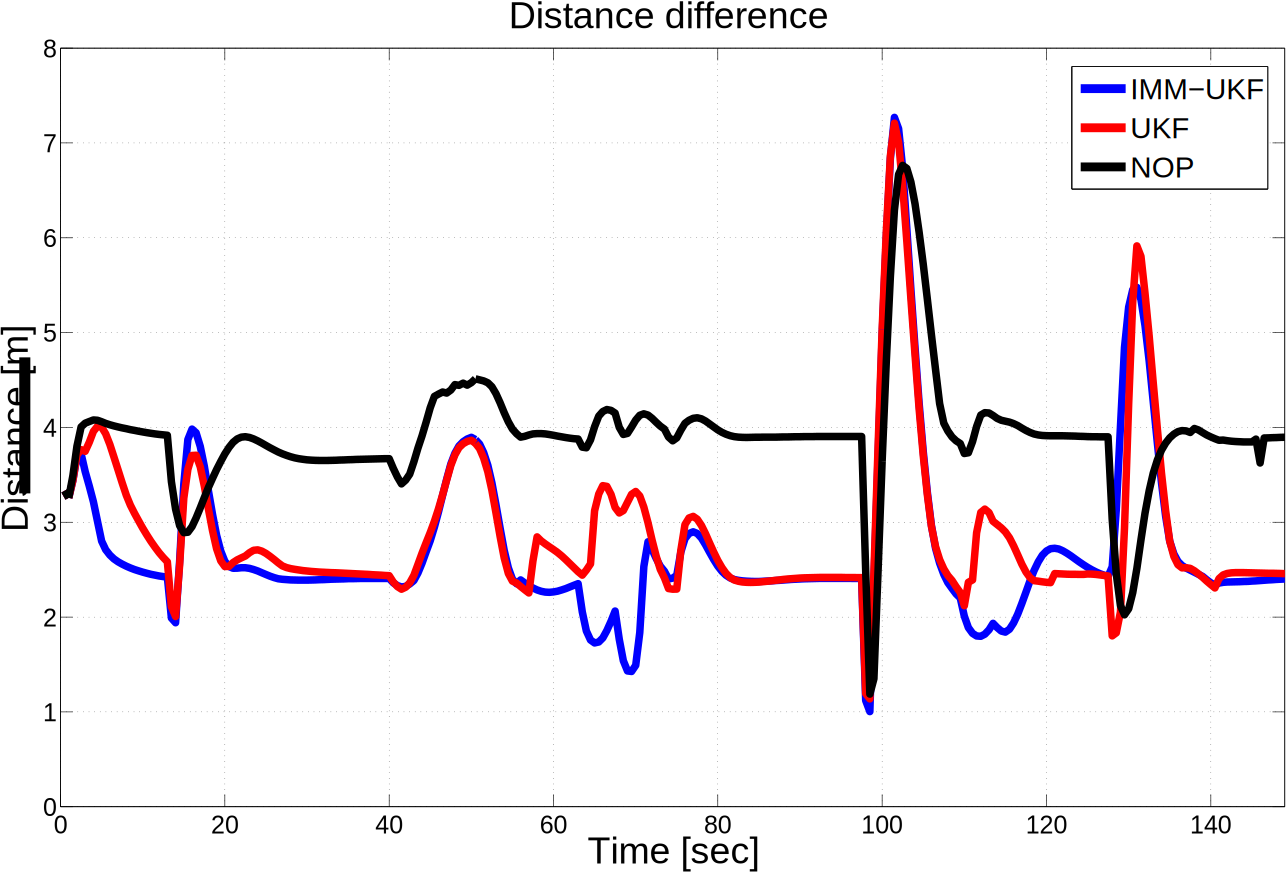
\includegraphics[width=0.4\textwidth]{figures/dis_diff2.pdf}
% 		\caption{Comparison of distance between the human and the robot using the MPC and the reactive methods}
% 		\label{fig:err_d}
% 	\end{figure}
	
% 	\begin{figure}
% 		\centering
% 		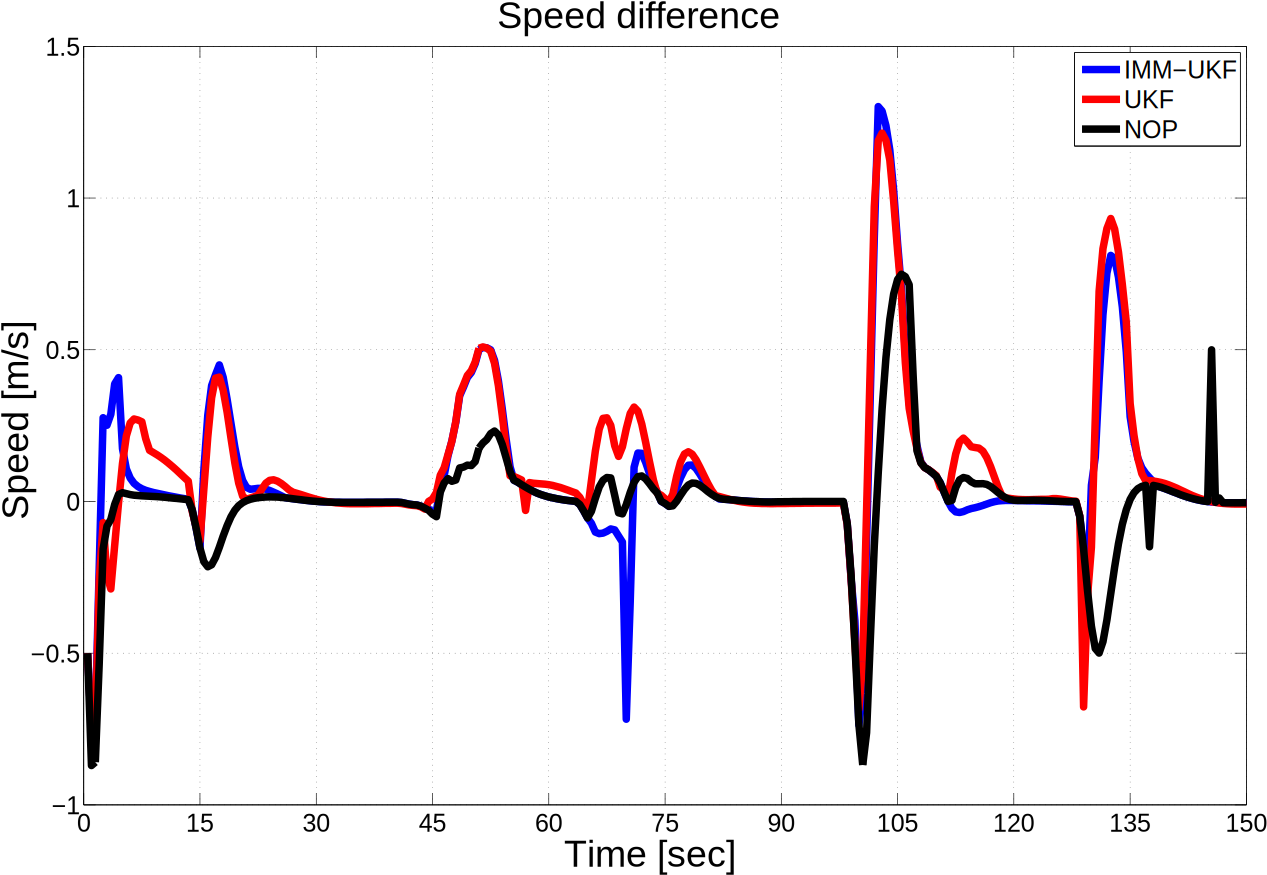
\includegraphics[width=0.4\textwidth]{figures/vel_diff2.pdf}
% 		\caption{Comparison of velocity difference between the human and the robot using the MPC and the reactive methods}
% 		\label{fig:err_v}
% 	\end{figure}
        \begin{figure} [t]
\centering	\includegraphics[width=0.43\textwidth]{figures/ddf}
		\caption{Comparison of the distance difference between the human and the robot for another scenario}
		\label{fig:constraint_violation}
\end{figure}	\section{CONCLUSION}\label{sec:conclusion}
	We have developed an autonomous motion planning framework for human-companion robots to accompany a target person in a socially desirable manner.
	Such companion robot can be useful for SAR scenarios by assisting humans in carrying apparatus, exploring dangerous areas or detecting survivors.
%    The dual IMM-UKF approach that incorporates the uniform motion model and the coordinated turn motion models is proposed for human motion estimation and prediction.
% 	The IMM-UKF approach that incorporates the uniform motion model and the coordinated turn motion models is proposed for human motion estimation and prediction.
	%Such multiple-model approach captures different human motion patterns, thus improving the estimation and prediction accuracy than other single-model approaches.
% 	Such multiple-model approach captures different human motion patterns, thus able to obtain accurate estimation and prediction.
%	Such multiple-model approach captures different human motion patterns, thus able to obtain 	accurate estimation. 
%	Moreover, the disturbance estimation based on IMM-UKF framework improves the prediction of human motion by providing the model mismatch.
	A Parallel Interacting Multiple Model-Unscented Kalman Filter (PIMM-UKF) approach
    %Parallel IMM-UKF approach 
    is proposed for the human motion prediction. 
    It combines two independent IMM-UKF estimators to estimate the human motion states and model mismatch simultaneously.
    Both IMM-UKF estimators incorporate the uniform motion model and the coordinated turn motion model to allow the mixed system dynamics. 
	Moreover, a corrective term provided from model mismatch estimator is added into human motion prediction.
%    into the process of human states prediction. 
        Such prediction framework captures different human motion patterns and the unmodeled dynamics, thus being able to obtain more accurate prediction.
% 	\clnote{
% 		We propose a dual IMM-UKF approach that incorporates the uniform motion model and the coordinated turn motion model for human motion estimation and prediction.
% 		Moreover, a novel disturbance estimation is devised based on the IMM-UKF framework, which significantly improves the prediction of human motion by adding a corrective term into the predicted human states.
% 		Such prediction framework captures different human motion patterns and unmodeled dynamics, thus being able to obtain accurate prediction.}
	Based on the predicted results, the model predictive control (MPC) is used to plan the robot's trajectory. Both the safety and comfort requirements are formulated into a finite-horizon constrained optimal control problem.
	%	The estimation and prediction performance using IMM-UKF is compared with LFK, UKF and IMM-LKF.
% 	Simulation results show superior performance in terms of the accuracy and response time in the estimation and prediction using the IMM-UKF approach compared to other three approaches: LKF, IMM-LKF and UKF, especially when the human makes curved motion or sharp turns.

	The proposed motion planning framework is evaluated using $10$ randomly generated SAR scenario in the simulations.
	The results show superior performance in terms of the accuracy and response time in the estimation and prediction using PIMM-UKF approach compared to IMM-UKF and each
    single model based-UKF methods, especially when the human makes curved motion or sharp turns.
	Moreover, the MPC planner is evaluated using the PIMM-UKF and non-prediction methods.
	The planner successfully ensures the safety of the accompanied person using these two prediction strategies, but the PIMM-UKF results in a better robot motion behavior by keeping the robot within the comfort zone from the human.
	%	The MPC motion planning approach is compared with a reactive method and shows that the MPC method achieves better performance in generating smaller human-robot distance while similar performance in the velocity difference.
	% The reactive policy achieves smaller velocity differences than the MPC method.
	% However, this becomes less attractive as the resultant human-robot distance becomes very large.
	
	In the future work, we plan to compare other motion prediction methods, such as the auto-regressive moving-average (ARMA) method, with PIMM-UKF approach.
	Besides, enabling the robot to learn human motion model in real time is an attractive topic, and may provide more accurate human motion prediction and results in better human-companion behavior.
	%%%%%%%%%%%%%%%%%%%%%%%%%%%%%%%%%%%%%%%%%%%%%%%%%%%%%%%%%%%%%%%%%%%%%%%%%%%%%%%%
	
	%\appendix
	\section*{APPENDIX}
	\subsection{Model Mismatch Estimation}
    The IMM-UKF approach is extended to estimate the model mismatch to improve the prediction of human motion. Two different augmented kinematic models containing model mismatch as states are utilized in IMM framework. The coordinated turn motion model for the model mismatch estimation is shown below:
	\begin{subequations}
		\begin{align*}
			x_{d,k+1}^{h,1}&= f^1_d(x_{d,k}^{h,1})+G_dw_{1,k} \\ 
			%Q(k)&=E[w(k)w(k)^\top]
			f_d(x_{d,k}^{h,1})&=\left[
			\begin{array}{c}
				p^h_1+\frac{\sin(\omega^h T)}{\omega^h}v^h_1-\frac{1-\cos(\omega^h T)}{\omega^h}v^h_2+\frac{T^2}{2}d^h_1\\
				\cos(\omega^h T)v^h_1-\sin(\omega^h T)v^h_2+Td^h_1\\
				p^h_2+\frac{1-\cos(\omega^h T)}{\omega^h}v^h_1+\frac{\sin(\omega^h T)}{\omega^h}v^h_2+\frac{T^2}{2}d^h_2\\
				\sin(\omega^h T)v^h_1+\cos(\omega^h T)v^h_2+Td^h_2\\
				\omega^h+Td^h_3\\
                d^h_1\\
                d^h_2\\
                d^h_3
			\end{array}\right] \\
			G_d &= \left[
			\begin{array}{cccccc}
				\frac{T^2}{2}& 0& 0&0 &0 &0\\
				T& 0& 0& 0& 0& 0\\
				0& \frac{T^2}{2}& 0& 0& 0& 0\\
				0& T& 0& 0& 0& 0\\
				0& 0& 1& 0& 0& 0\\ 
                0& 0& 0& T& 0& 0\\
                0& 0& 0& 0& T& 0\\
                0& 0& 0& 0& 0& T\\
%             G^T &= \left[
% 			\begin{array}{ccccc}
% 				\frac{T^2}{2}& T & 0 & 0& 0\\
% 				0 & 0 & \frac{T^2}{2} & T & 0\\
% 				0& 0 & 0 & 0 & 1\\
			\end{array}\right] \\
			w_1&\sim\mathcal{N}(0,Q^1_d).
		\end{align*}
	\end{subequations}\normalsize
	
	The equation of the uniform motion for the model mismatch estimation is represented as follows:
	\begin{subequations}
		\begin{align*}
			x_{d,k+1}^{h,2}&= f_d^2x_{d,k}^{h,2}+G_dw_{2,k} \label{eqn:h_d_dyn}\\
            f_d^2(x_{s,k}^{h,2})&=\left[
			\begin{array}{c}
				p^h_1+v^h_1T+\frac{T^2}{2}d^h_1\\
				v^h_1+Td^h_1\\
				p^h_2+v^h_2T+\frac{T^2}{2}d^h_2\\
				v^h_2+Td^h_2\\
				\omega^h+Td^h_3\\ 
                d^h_1\\
                d^h_2\\
                d^h_3
			\end{array}\right] \\             
% 			A_d&=\left[
% 			\begin{array}{cccccccc}
% 				1& T& 0& 0& 0& \frac{T^2}{2}& 0& 0\\
% 				0& 1& 0& 0& 0& T& 0& 0\\
% 				0& 0& 1& T& 0& 0& \frac{T^2}{2}& 0\\
% 				0& 0& 0& 1& 0& 0& T& 0\\
% 				0& 0& 0& 0& 0& 0& 0& T\\
% 			\end{array}\right]\\
% 			B&=\left[
% 			\begin{array}{ccc}
% 				\frac{T^2}{2}& 0& 0\\
% 				T& 0& 0\\
% 				0& \frac{T^2}{2}& 0\\
% 				0& T& 0\\
% 				0& 0& 1\\
% 			\end{array}\right] \\
			w_2&\sim\mathcal{N}(0,Q^2_d),
		\end{align*}
	\end{subequations}\normalsize
	where $x_{d,k}^{h,i}$, $i=1,2$ represents the human motion state including eight elements in the model mismatch estimation: $p^h_1,v^h_1,p^h_2,v^h_2,\omega^h,d^h_1,d^h_2,d^h_3$, where 
%     $p^h_1,p^h_2$ denote the longitudinal and lateral position of the human, $v^h_1,v^h_2$ the corresponding velocity, $\omega^h$ the turn rate of the human 
the first five states are defined as in \cref{subsec:human_track}, and $d^h_1,d^h_2,d^h_3$ represent the model mismatch of longitudinal, lateral and angular directions, respectively; $w_{i,k}$, $i=1,2$ represents process noise that follows a zero-mean Gaussian distribution with $Q^i_d$ being the covariance matrix.
    
	The observation model for the model mismatch estimation is represented as : 
\addtocounter{equation}{-3}
\begin{equation}
		y_{d,k}^h=C_dx_{d,k}^h+v_k,\label{eqn:nd_observation}
	\end{equation}
	where $y_{d,k}^h$ denotes the observed human state at the time step $k$; $v_k$ stands for measurement noise. 
	
	By using GPS or camera sensors, the human positions can be directly measured.
	Therefore, the parameters in observation model \cref{eqn:nd_observation} is defined as:

   \begin{subequations}
		\begin{align*}
			C_d&=\left[
			\begin{array}{cccccccc}
				1& 0& 0& 0& 0& 0& 0& 0\\
				0& 0& 1& 0& 0& 0& 0& 0
			\end{array}\right],
			v\sim\mathcal{N}(0,V_d),
		\end{align*}
	\end{subequations}\normalsize
	where $V_d$ is the convariance matrix of the measurement noise.	
% 	\subsection{IMM-LKF Method}
% 	Similar to IMM-UKF, IMM-LKF works with two motion models: the uniform motion model and the coordinated turn motion model. If the turn rate is a known constant in the coordinated turn motion model, the human estimation procedure can be modeled with the discrete time linear system as follows:
% \small	\begin{subequations}
% 		\begin{align}
% 			x^h(k+1) = Ax^h(k)+B_ww(k)\label{eqn:h_dyn}\\
% 			y^h(k)=Cx^h(k)+v(k)\label{eqn:observation}
% 		\end{align}
% 	\end{subequations}
%     \normalsize
% 	where $x^h(k)$ and $y^h(k)$ represent the human motion state and the observation, respectively, at the time step $k$; $w(k)$ and $v(k)$ represent process noise and measurement noise, respectively.
% 	$x^h(k)$ consists of four elements: $p^h_1,v^h_1,p^h_2,v^h_2$, where $p^h_1,p^h_2$ denote the longitudinal and lateral position of the human and $v^h_1,v^h_2$ the corresponding velocity.
% 	We use two LKFs in the IMM for human tracking, each corresponding to a different kinematic model: the uniform motion model and the turn motion model.
% 	Two models differ in the $A$ matrix and $w$ in \cref{eqn:h_dyn} while sharing the same $B_w$.
% 	In particular, we define the matrices as follows:
% \small\begin{subequations}
% \begin{align*}
% 			A_U&=\left[
% \scriptsize\begin{array}{cccc}
% 				1& T& 0& 0\\
% 				0& 1& 0& 0\\
% 				0& 0& 1& T\\
% 				0& 0& 0& 1
% 			\end{array}\right],
% 			A_T=\left[
% \scriptsize\begin{array}{cccc}
% 				1& \frac{\sin(\omega T)}{\omega}& 0& \frac{1-\cos(\omega T)}{\omega}\\
% 				0& \cos(\omega T)& 0& -\sin(\omega T)\\
% 				0& \frac{1-\cos(\omega T)}{\omega}& 1& \frac{\sin(\omega T)}{\omega}\\
% 				0& \sin(\omega T)& 0& \cos(\omega T)
% 			\end{array}\right]\\
% 			B_w&=\left[
% \scriptsize\begin{array}{cccc}
% 				\frac{T^2}{2}& T& 0& 0\\
% 				0& 0& \frac{T^2}{2}& T
% 			\end{array}\right],
% 			w_U\sim\mathcal{N}(0,Q_U),\; w_T\sim\mathcal{N}(0,Q_T)
% 		\end{align*}
% 	\end{subequations}\normalsize
% 	where $A_U$ and $A_T$ stand for the $A$ matrices of the uniform motion model and turn motion model, respectively; $w_U$ and $w_T$ denote the process noise of the uniform motion model and turn motion model, respectively; $T$ represents the sampling time; $\omega$ represents the constant turn rate.
	
% 	We assume that only the human position can be measured.
% 	Therefore, the parameters in observation model \cref{eqn:observation} can be defined as:
% 	\small\begin{subequations}
% \scriptsize\begin{align*}
% 			C=\left[
% 			\begin{array}{cccc}
% 				1& 0& 0& 0\\
% 				0& 0& 1& 0
% 			\end{array}\right],
% 			v\sim\mathcal{N}(0,V)
% 		\end{align*}
% 	\end{subequations}\normalsize
% % 	Above linear state space models are used in LKF and IMM-LKF in this paper.
% 	Moreover, we set the turn rate $\omega$ to be $0.1$ rad/s as a known constant, in the turn motion model in IMM-LKF. 
	
	\subsection{Approximating Static Obstacles}\label{subsec:ellip_approx}
%     \begin{figure}
% 		\centering		
% 		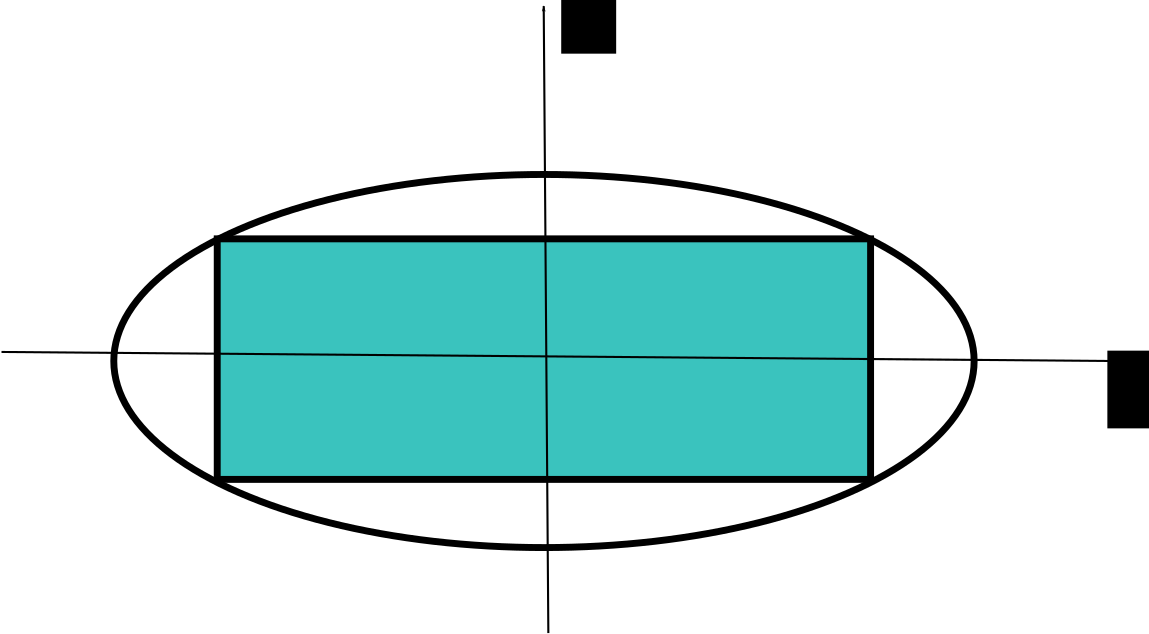
\includegraphics[width=0.3\textwidth]{figures/approx_ellipse}
% 		\caption{Approximating the rectangle obstacle with an ellipse.}
% 		\label{fig:approx_ellipse}
% 	\end{figure}
    
	Static rectangular obstacles are approximated and analytically represented as ellipses. %, as shown in \cref{fig:approx_ellipse}.
	Let $a$ and $b$ be the length and width of a rectangular obstacle centered at the origin.
	Let \cref{eqn:ellipse} represent the ellipse that encloses the obstacle in the way that the four vertices of the rectangle lie on the boundary of the ellipse:
\addtocounter{equation}{-1}
	
	\begin{equation}\label{eqn:ellipse}
		\frac{x^2}{\alpha^2}+\frac{y^2}{\beta^2}=1.
	\end{equation}
	In addition, assume that the rectangle and ellipse have the same aspect ratio, which means $\frac{a}{b}=\frac{\alpha}{\beta}$, then by simple algebraic manipulation, we can obtain that $\alpha=\frac{a}{\sqrt{2}}$ and $\beta=\frac{b}{\sqrt{2}}$.
	Define $h(x,y)=2\frac{(x-c_1)^2}{a^2}+2\frac{(y-c_2)^2}{b^2}-1.$
%\small	\begin{equation*}
%		h(x,y)=2\frac{x^2}{a^2}+2\frac{y^2}{b^2}-1.
%	\end{equation*} \normalsize
	The $h(x,y)=0$ represent the shifted-center ellipse approximation of the rectangle with length $a$ and width $b$.
	Any point $(x,y)$ with $h(x,y)>0$ lies outside of the ellipse. \cref{fig:approx_ellipse} shows the schematic plot of the approximating ellipse for the rectangular obstacle centered at $(c_1,c_2)$.
 	\begin{figure}[h]
 		\centering		
 		\includegraphics[width=0.32\textwidth]{figures/ellipse}
 		\caption{Approximating the rectangle obstacle with an ellipse.}
 		\label{fig:approx_ellipse}
 	\end{figure}		
% 	\begin{figure}
% 		\centering		
% 		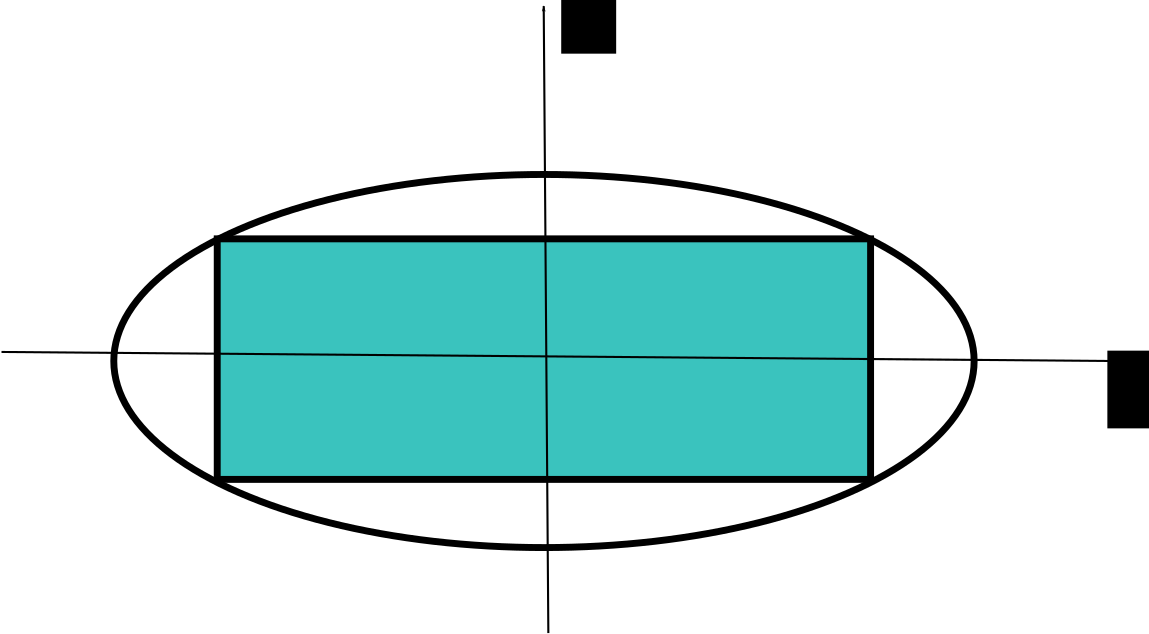
\includegraphics[width=0.25\textwidth]{figures/approx_ellipse}
 %		\caption{Approximating the rectangle obstacle with an ellipse.}
% 		\label{fig:approx_ellipse}
% 	\end{figure}
	
	
	
	\addtolength{\textheight}{-10cm}   % This command serves to balance the column lengths
	% on the last page of the document manually. It shortens
	% the textheight of the last page by a suitable amount.
	% This command does not take effect until the next page
	% so it should come on the page before the last. Make
	% sure that you do not shorten the textheight too much.
	
	
	%%%%%%%%%%%%%%%%%%%%%%%%%%%%%%%%%%%%%%%%%%%%%%%%%%%%%%%%%%%%%%%%%%%%%%%%%%%%%%%%
	
\bibliographystyle{ieeetr}
\bibliography{references}
    
% \begin{IEEEbiography}{Donghan Lee}
% Biography text here.
% \end{IEEEbiography}

% % if you will not have a photo at all:
% \begin{IEEEbiographynophoto}{John Doe}
% Biography text here.
% \end{IEEEbiographynophoto}

% % insert where needed to balance the two columns on the last page with
% % biographies
% %\newpage

% \begin{IEEEbiographynophoto}{Jane Doe}
% Biography text here.
% \end{IEEEbiographynophoto}

\end{document}